\documentclass[aps,prd,nofootinbib,amsmath,amssymb,superscriptaddress,twocolumn,10pt]{revtex4}%superscriptaddress,showpacs,

\pdfoutput=1



%\usepackage{txfonts}
\usepackage{graphicx}
\usepackage{dcolumn}
\usepackage{bm}
\usepackage{amssymb}
%\usepackage{latexsym}
\usepackage{booktabs}
\usepackage{amsmath}
\usepackage{multirow}
\usepackage[colorlinks=true, linkcolor=purple, citecolor=blue]{hyperref}

\newcommand{\be}{\begin{equation}}
\newcommand{\ee}{\end{equation}}
\newcommand{\bq}{\begin{eqnarray}}
\newcommand{\eq}{\end{eqnarray}}
%\def\be{\begin{equation}}
%\def\ee{\end{equation}}
%\def\ba{\begin{eqnarray}}
%\def\ea{\end{eqnarray}}
\def\half{\frac{1}{2}}
\def\nn{\nonumber}


\newcommand{\mnras}{Mon. Not. R. Astron. Soc.}
\newcommand{\apjl}{Astrophys. J. Lett.}
\newcommand{\apjs}{Astrophys. J. Supp.}
\newcommand{\epspar}{\epsilon}
\newcommand{\thepar}{\theta}
\newcommand{\Bpar}{B}
\newcommand{\Epar}{E}
\newcommand{\mA}{{\cal A}}
\newcommand{\mB}{{\cal B}}
\newcommand{\ds}{\mathrm{d}}
\newcommand{\red}{\textcolor[rgb]{1.00,0.00,0.00}}

\newcommand{\potential}{{A}}
\newcommand{\shift}{{B}}
\newcommand{\curvature}{{H}_L}
\newcommand{\shear}{{H}_T}
\newcommand{\kh}{k_H}
\newcommand{\ck}{c_K}
\newcommand{\tppi}{\ck p_T \Pi_T}


\bibliographystyle{unsrt}
\DeclareMathOperator{\sgn}{sgn}
\usepackage[usenames,dvipsnames]{xcolor}

\begin{document}


\title{Quantifying the impacts of future gravitational-wave data on constraining interacting dark energy}

\author{Hai-Li Li}
\affiliation{Department of Physics, College of Sciences, Northeastern
University, Shenyang 110819, China}
\author{Dong-Ze He}
\affiliation{Department of Physics, College of Sciences, Northeastern
University, Shenyang 110819, China}
\author{Jing-Fei Zhang}
\affiliation{Department of Physics, College of Sciences, Northeastern
University, Shenyang 110819, China}
%\author{}
%\affiliation{Department of Physics, College of Sciences, Northeastern University, Shenyang 110819, China}

\author{Xin Zhang\footnote{Corresponding author}}
\email{zhangxin@mail.neu.edu.cn}
\affiliation{Department of Physics, College of Sciences, Northeastern
University, Shenyang 110819, China}
\affiliation{Ministry of Education Key Laboratory of Data Analytics and Optimization
for Smart Industry, Northeastern University, Shenyang 110819, China}
\affiliation{Center for High Energy Physics, Peking University, Beijing 100080, China}
\date{\today}

\begin{abstract}
In this work, we investigate the impacts of the gravitational-wave (GW) standard siren observation of the Einstein Telescope (ET) on constraining the interacting dark energy models. We simulate 1000 GW events data in the redshift range  $0\lesssim z \lesssim 5$ based on the 10 years observation of the ET. We combine the simulated GW data with the current mainstream cosmological electromagnetic observations including the cosmic microwave background (CMB) anisotroties observation, the baryon acoustic oscillations (BAO), and the type Ia supernovae (SN) observation (Pantheon compilation) to constrain these models. We consider two typical interacting dark energy (IDE) models, i.e., the I$\Lambda$CDM model and I$w$CDM model, in the context of a perturbed universe. To avoid the large-scale instability problem for IDE models, we apply the parameterized post-Friedmann (PPF) approach to do the analysis. We find that the addition of GW standard siren data could improve the constraint accuracies on most of the cosmological parameters (e.g., $H_{0}$, $w$, and $\Omega_{\rm m}$) significantly. \red{For the coupling constant $\beta$, the absolute constraint errors could also be slightly improved when adding the GW data in the cosmological fit}.

%model of vacuum energy interacting with cold dark matter (I$\Lambda$CDM) and the interacting $w$ cold dark matter (I$w$CDM) model
\end{abstract}
%\pacs{95.36.+x, 98.80.Es, 98.80.-k}
\maketitle

%\pacs{95.36.+x, 98.80.Es, 98.80.-k} \maketitle
\section{Introduction}\label{sec1}

The accelerated expansion of Universe, discovered by the observations of type Ia supernovae \cite{Riess:1998cb,Perlmutter:1998np} and further confirmed by the observations of cosmic microwave background \cite{Spergel:2003cb,Bennett:2003bz} and large scale structure \cite{Tegmark:2003ud,Abazajian:2004aja}, has become a fact.
%Since then, cosmologists have begun to pay attention to investigate the accelerated expansion of the universe.
In order to explain the cosmic acceleration, the concept of ``dark energy'',  which is an exotic form of energy with negative pressure and provides repulsive force, has been proposed \cite{Sahni:2006pa,Bamba:2012cp,Weinberg:1988cp,Peebles:2002gy,Copeland:2006wr,Frieman:2008sn,Sahni:2008zz,Li:2011sd,Kamionkowski:2007wv}. At present, dark energy (DE) occupies about 68\% of the total energy density of cosmos, dominating the evolution of our current universe significantly.

The cosmological constant $\Lambda$, proposed by Einstein in 1917, has always been regarded as the simplest candidate of DE until now. The combination of cosmological constant $\Lambda$ (or vacuum energy) and cold dark matter (CDM) constitute a concordance cosmological prototype, which is also called the $\Lambda$CDM model. The equation of state (EoS) parameter of vacuum energy is $w_{\Lambda} \equiv p_{\Lambda}/\rho_{\Lambda}=-1$. Although the $\Lambda$CDM model is in excellent agreement with current cosmological observations with the least parameters \cite{Ade:2015xua}, the cosmological constant $\Lambda$ has always been bothered by some severe theoretical puzzles, such as the ``fine-tuning'' and ``cosmic coincidence'' problems \cite{Sahni:1999gb,Bean:2005ru}. Thus, it is hard to say that the cosmological constant model with only six primary parameters is the final scenario of our universe, which implies that the $\Lambda$CDM model is necessary to be further extended and some new physics maybe exist in the extensions.

To extend the $\Lambda$CDM cosmology on the aspect of DE, there are mainly two possible theoretical orientations, i.e., dynamical dark energy and modified gravity (MG) theories. If Einstein's general relativity (GR) is valid on all the scales of Universe, an alternative proposal of $\Lambda$ is dynamical dark energy, which suggests that the energy form with negative pressure can be provided by a spatially homogeneous scalar field evolving slowly down a proper potential, dubbed quintessence. On the other hand, if GR could break down on the cosmological scales, some models of MG can mimic the ``effective dark energy" at the cosmological background level to explain the cosmic accelerated expansion. In general, a dynamical DE model, compared to the cosmological constant, can yield a different expansion history of the universe but a similar growth history of structure. On the contrary, the MG models can yield a similar expansion history but a quite different structure growth history. Discriminating the scenarios of dynamical DE and MG has become one of the most critical issues in modern cosmology.

However, it must be stressed out that there is another important theoretical possibility that dark energy and dark matter can directly interact with each other, through mediating some unknown scalar field degrees of freedom, also called ``the fifth force". Inspired by this possibility, a large number of models featuring the interactions between dark matter and dark energy have been constructed and researched \cite{Amendola:1999er,Amendola:1999qq,TocchiniValentini:2001ty,Amendola:2001rc,Comelli:2003cv,Chimento:2003iea,Cai:2004dk,Zhang:2004gc,Ferrer:2004nv,Zimdahl:2005bk,Zhang:2005rj,Wang:2006qw,Sadjadi:2006qp,Barrow:2006hia,Sasaki:2006kq,Abdalla:2007rd,Bean:2007ny,Guo:2007zk,Bertolami:2007zm,Boehmer:2008av,He:2008tn,CalderaCabral:2008bx,Bean:2008ac,Szydlowski:2008by,Chen:2008ft,Valiviita:2008iv,Couderc:2009tq,Chimento:2009hj,CalderaCabral:2009ja,Majerotto:2009np,Valiviita:2009nu,He:2009mz,He:2009pd,Koyama:2009gd,Li:2009zs,Xia:2009zzb,Cai:2009ht,He:2010ta,Cui:2010dr,Li:2010eu,Gavela:2010tm,Martinelli:2010rt,He:2010im,Chen:2011rz,Fu:2011ab,Clemson:2011an,Li:2011ga,Xu:2011tsa,Zhang:2012uu,Xu:2013jma,Zhang:2013zyn,Wang:2013qy,Salvatelli:2013wra,Yang:2014gza,yang:2014vza,Wang:2014oga,Faraoni:2014vra,Yin:2015pqa,Fan:2015rha,Cai:2015zoa,Duniya:2015nva,Feng:2016djj,Murgia:2016ccp,Sola:2016jky,Sola:2016ecz,Sola:2016zeg,Pourtsidou:2016ico,Costa:2016tpb,Xia:2016vnp,vandeBruck:2016hpz,Kumar:2016zpg,Kumar:2017dnp,Santos:2017bqm,Sola:2017jbl,Guo:2017hea,Zhang:2017ize,Feng:2018yew,Yang:2018euj,Zhao:2018fjj,Li:2019loh}.
Although the interaction between dark matter and dark energy is mild, we still cannot exclude it within $1\sigma$ confidence region \cite{Costa:2013sva,Salvatelli:2014zta,Nunes:2016dlj, Abdalla:2014cla,Yang:2017ccc,Yang:2017zjs,Li:2018ydj,Feng:2019mym}. What is important is that the models of interacting dark energy can successfully solve  (or alleviate) the fine-tuning and coincidence problems through the attractor solution. Furthermore, the interation between dark matter and dark energy not only can alleviate the tension in the values of Hubble constant $H_{0}$ originated from its local and global measurements \cite{Guo:2018ans}, but also can explain the excess amount of 21 cm absorption signal around the redshift $z \sim 17$ detected by the Experiment to Detect the Global Epoch of Reionization Signature (EDGES) \cite{Costa:2018aoy,Xiao:2018jyl,Li:2019loh}. Thus, the research on the interacting dark energy model is expected to be importantly significant and valuable.

Currently, the major cosmological probes include the cosmic microwave background (CMB) anisotropies, baryon acoustic oscillations (BAO), type Ia supernovae (SN), direct determination of the Hubble constant ($H_{0}$), weak gravitational lensing (WL), redshift space distortions (RSD) etc. Some important cosmological parameters have been precisely measured by the combination of these electromagnetic (EM) probes. But for the parameters beyond the standard model, such as the EOS of dark energy, the sterile neutrino mass, the tensor-to-scalar ratio and so forth, we still cannot measure them accurately up to now. In fact, there are strong degeneracies between these parameters, and some conflicts also exist among various observations. The reason for the situation is that, the current observation are still not accurate enough so that we can not precisely measure the cosmological parameters beyond the standard model. In order to better constrain these parameters, we also need some new cosmological probes other than the traditional optical cosmological probes.

As proposed by Schutz in 1986 \cite{Schutz:1986gp} and subsequently discussed by Holz and Hughes \cite{Holz:2005df}, the observations of the gravitation wave (GW) can be used as the \textit{standard sirens} in cosmology.
The detection of GW event GW170817 from the merge of binary neutron star (BNS) and its EM counterpart GRB170817A has pronounced the arrival of the multi-messenger astronomy era. With the help of the multi-messenger observation, we can measure the absolute luminosity distance $d_{\rm L}$ of the source from the gravitational wave signal as well as the redshift $z$ from the electromagnetic counterparts. Then, we can establish a true distance-redshift relation which can be used to infer the expansion history of universe and constrain the cosmological parameters such as Hubble constant \cite{Abbott:2017xzu}. The main advantage of the standard siren method is that it avoids using the cosmic distance ladder. Therefore, the future GW standard sirens would become a promising new cosmological probe, and would play a significant role in the cosmological parameter measurements.

Actually, in the near future, a planed third-generation ground-based GW detector, the Einstein Telescope (ET), will be brought into operation \cite{ET}. This impressive equipment will hold 10 km-long arms and three detectors. Compared with the advanced LIGO, it has a much wider detection frequency range and a much better detection sensitivity. Thus, there will be much more BNS events in much deeper redshifts detected by ET. As a conservative estimation, at least 1000 useful standard siren events data will be observed with ET's ten years operation \cite{Zhang:2018byx}.
In some previous works \cite{Zhao:2018gwk,Du:2018tia,Zhang:2018byx,Zhang:2019ple,Yang:2019bpr,Yang:2019vni,Bachega:2019fki,Zhang:2019loq,Zhang:2019ylr,Chang:2019xcb,He:2019dhl}, the authors have already utilized the GW standard siren observation to estimate the cosmological parameters in many various cosmological models. For example, in Ref. \cite{Zhang:2018byx} the authors have investigated the capability of future GW standard siren observation on improving the parameter estimation in cosmology and breaking the parameter degenracies formed in traditional EM observations. Taking ET as an example, they simulated 1000 events data based on the ten years observation and find that, the simulated GW data could largely break the parameter degeneracy in $\Lambda$CDM model as well as $w$CDM model, significantly improving the parameter constraints in the cosmological fit. In Ref. \cite{Zhang:2019loq}, the authors have also investigated the Chevalliear-Polarski-Linder (CPL) model, $\alpha$ dark energy ($\alpha$DE) model, generalized Chaplygin gas (GCG) model and new generalized Chaplygin gas (NGCG) model with the simulated GW standard siren data, and GW data could also improve the constraints on the cosmological parameters for all these DE models. Likewise, the similar conclusion was also obtained for the holographic dark energy (HDE) models in Ref. \cite{Zhang:2019ple}. 

\red{As for the interacting dark energy (IDE) models, Yang et al. \cite{Yang:2019vni} have investigated how the future GW data could help improve the limits on the parameters in I$\Lambda$CDM models, finding that the addition of GW data can reduce the current uncertainty by a factor of 5. 
In this work, we will further explore the impacts of the future GW data on improving the parameter constraints or breaking the parameter degeneracy for extensive IDE models (e.g., I$\Lambda$CDM model and I$w$CDM model).}
We consider another two cases of energy transfer rate, i.e., $Q=\beta H \rho_{\rm c}$ and $Q=\beta H_{0} \rho_{\rm c}$, where $\rho_{\rm c}$ is the energy density of cold dark matter. In order to treat the cosmological perturbation evolution in these models, we employ the parameterized post-Friedmann (PPF) scheme for the IDE scenario \cite{Li:2014eha} to make the calculations. This work will make the analysis of the constraining power of future GW standard siren observation on cosmological parameters more general and complete.


This paper is organized as follows. In Sec.~\ref{sec2}, we give a brief description of the PPF approach in the interacting dark energy models. In Sec.~\ref{sec3}, we introduce the current standard cosmological data and briefly describe the method to simulate the gravitational wave data. In Sec.~\ref{sec4}, we report the constraint results and make some relevant discussions for them. Conclusion is given in Sec.~\ref{sec5}.


\section{A brief description of the PPF approach for the interacting dark energy models}\label{sec2}

If there is a direct, non-gravitational interaction between dark energy and dark matter, we will have the following energy continuity equations
\begin{align}
&\rho'_{\rm de} = -3\mathcal{H}(1+w)\rho_{\rm de}+ aQ_{\rm de},\label{eq1}\\
&\rho'_{\rm c} = -3\mathcal{H}\rho_{\rm c}+aQ_{\rm c},~~~~~~Q_{\rm de}=-Q_{\rm c}=Q,\label{eq2}
\end{align}
where $\rho_{\rm de}$ and $\rho_{\rm c}$ are the energy densities of dark energy and dark matter; a prime is the derivative with respect to the conformal time $\eta$; $\mathcal{H}=a'/a$ is the conformal Hubble expansion rate; $a$ denotes the scale factor; $w$ is the EoS parameter; and $Q$ is the phenomenological interaction term. Generally, the form of $Q$ is assumed to be proportional to the density of dark sectors, and it can include the Hubble parameter $H$ or the Hubble constant $H_{0}$. In this paper, we consider two forms about the $Q$, e.g., $Q=\beta H \rho_{\rm c}$, $Q=\beta H_{0} \rho_{\rm c}$,  with $\beta$ being a dimensionless coupling parameter used to describe the interacting strength between dark energy and dark matter. From Eqs. (\ref{eq1}) and (\ref{eq2}), we can clearly find that if $\beta>0$, dark matter decays into dark energy, and vice versa for $\beta<0$. Here, $\beta=0$ denotes no interaction between the two sectors.


The covariant conservation law of the dark sectors can be expressed as
\begin{equation}
\label{eqn:energyexchange} \nabla_\nu T^{\mu\nu}_I = Q^\mu_I, \quad\quad
 \sum_I Q^\mu_I = 0,
\end{equation}
where $T^{\mu\nu}_I$ is the energy-momentum tensor, and $Q^\mu_I$ is the energy-momentum transfer vector. In this paper, we choose $Q^\mu_{\rm de}=-Q^\mu_{\rm c}=Qu^\mu_{\rm c}$, where $u^\mu_{\rm c}$ is the four-velocity of dark matter. The energy-momentum transfer vector $Q^\mu_I$ can be split into two parts as
\begin{equation}
Q^I_\mu  = a\big( -Q_I(1+AY) - \delta Q_IY,\,[ f_I+ Q_I (v-B)]Y_i\big),\label{eq:Qenergy}
\end{equation}
where $\delta Q_I$ is the energy transfer perturbation and $f_I$ is the momentum transfer potential of the $I$ fluid. $A$ and $B$ are the scalar metric perturbations. $Y$ is the eigenfunctions of the Laplace operator ($\nabla^{2}Y=-k^{2}Y$) and $Y_i$ is the covariant derivative ($Y_{i}=(-k)\nabla_{i}Y$).

In the interacting dark energy models, we can give the following conservation equations for the $I$ fluid according to Equations~(\ref{eqn:energyexchange}) and (\ref{eq:Qenergy}),
\begin{equation}
 {\delta\rho_I'}
	+  3\mathcal{H}({\delta \rho_I}+ {\delta p_I})+(\rho_I+p_I)(k{v}_I + 3 H_L')=a(\delta Q_I+AQ_I),\label{eqn:conservation1}
\end{equation}	
\begin{align}	
[(\rho_{I}+p_{I})(v_{I}-B)]'+4\mathcal{H}(\rho_I + p_I)({{v_I}-{B}})-k{ \delta p_I }\nonumber \\
+\frac{2}{3}kc_{K} p_I {\Pi_I}- k(\rho_I+ p_I) {A}=a[Q_I(v-B)+f_I],\label{eqn:conservation2}
\end{align}
In the equations above, $\delta\rho_I$ is the energy density perturbation, $\delta p_I$ is the isotropic pressure perturbation, $v_I$ is the velocity perturbation, and $c_K = 1-3K/k^2$ with $K$ being the spatial curvature, and $\Pi_I$ is the anisotropic stress perturbation.

When considering the interaction between dark matter and dark energy, dark energy is treated as a nonadiabatic fluid and the calculation of $\delta p_{\rm de}$ is in terms of the adiabatic sound speed and the rest-frame sound speed. Under such circumstances, the interacting dark energy models will be confused with the problem of large-scale instability. Hence, we should treat the dark energy perturbations under the generalized PPF framework~\cite{Li:2014eha}. For clarity, in the following discussion, we will use some new symbols, i.e., $\zeta\equiv H_L$, $\xi\equiv A$, $\rho\Delta\equiv\delta\rho$, $\Delta p\equiv\delta p$, $V\equiv v$, and $\Delta Q_I\equiv\delta Q_I$, to denote the corresponding quantities of the comoving gauge, except the two gauge-independent quantities $\Pi$ and $f_I$.

On the large scales, the direct relationship between $V_{\rm de} - V_T$ and $V_T$ can be established, and it can be parametrized by a function $f_\zeta(a)$ as \cite{Hu:2008zd,Fang:2008sn}
\begin{equation}
\lim_{k_H \ll 1}\frac{4\pi G a^2}{\mathcal{H}^2}(\rho_{\rm de} + p_{\rm de})\frac{V_{\rm de} - V_T}{k_H}=-\frac{1}{3}ck_{K} f_\zeta(a) k_H V_T,\label{eq:DEcondition}
\end{equation}
where $k_H=k/\mathcal{H}$. The equation of motion for the curvature perturbation $\zeta$ on the large scales can be get by combining this equation with Einstein equations,
\begin{align}
\lim_{k_H \ll 1} \zeta'  = \mathcal{H}\xi - \frac{K}{k} V_T +\frac{1}{3} ck_{K}  f_\zeta(a) k V_T.
\label{eqn:zetaprimesh}
\end{align}
On the small scales, one can describe the evolution of curvature perturbation by using Poisson equation, $\Phi=4\pi G a^2\Delta_T \rho_T/( k^2\ck)$, with $\Phi=\zeta+V_T/k_H$. These two limits can be linked by the introduction of a dynamical function $\Gamma$,
\begin{equation}
\Phi+\Gamma = {4\pi Ga^2
\over  k^2\ck} \Delta_T \rho_T,
\label{eqn:modpoiss}
\end{equation}
which is satisfied for all the scales.

Compared with the small-scale Poisson equation, Eq.~(\ref{eqn:modpoiss}) gives $\Gamma\rightarrow0$ at $k_H\gg1$. Combining the derivative of Eq.~(\ref{eqn:modpoiss}) with the conservation equations and the Einstein equations, the equation of motion for $\Gamma$ on the large scales can be expressed as follows,
\begin{equation}\label{eq:gammadot}
\lim_{k_H \ll 1} \Gamma'  = S -\mathcal{H}\Gamma,
\end{equation}
with
\begin{align}
S&={4\pi Ga^2
\over k^2 } \Big\{[(\rho_{\rm de}+p_{\rm de})-f_{\zeta}(\rho_T+p_T)]kV_T \nonumber\\
&\quad+{3a\over k_Hc_K}[Q_{\rm c}(V-V_T)+f_{\rm c}]+\frac{a}{c_K}(\Delta Q_{\rm c}+\xi Q_{\rm c})\Big\},\nonumber
\end{align}
where $\xi$ can be obtained from Eq.~(\ref{eqn:conservation2}),
\begin{equation}
\xi =  -{\Delta p_T - {2\over 3}\tppi+{a\over k}[Q_{\rm c}(V-V_T)+f_{\rm c}] \over \rho_T + p_T}.
\label{eqn:xieom}
\end{equation}

By the transition scale parameter $c_\Gamma$, we can take the equation of motion for $\Gamma$ on all scales to be \cite{Hu:2008zd,Fang:2008sn}
\begin{equation}
(1 + c_\Gamma^2 k_H^2) [\Gamma' +\mathcal{H} \Gamma + c_\Gamma^2 k_H^2 \mathcal{H}\Gamma] = S.
\label{eqn:gammaeom}
\end{equation}

From Eq. (\ref{eqn:gammaeom}) we can see that in the equation of motion for $\Gamma$, all of the perturbation quantities contain only the matters and without dark energy. So, we can also solve Eq. (\ref{eqn:gammaeom}) without using any information related to the dark energy perturbations. As long as we know the evolution of $\Gamma$, we can get the energy density and velocity perturbations immediately,
\begin{align}
&\rho_{\rm de}\Delta_{\rm de} =- 3(\rho_{\rm de}+p_{\rm de}) {V_{\rm de}-V_{T}\over k_{H} }-{k^{2}\ck \over 4\pi G a^{2}} \Gamma,\\ \label{eqn:ppffluid}
& V_{\rm de}-V_{T} ={-k \over 4\pi Ga^2 (\rho_{\rm de} + p_{\rm de}) F} \nonumber \\
&\quad\quad\quad\times\left[ S - \Gamma' - \mathcal{H}\Gamma + f_{\zeta}{4\pi Ga^2 (\rho_{T}+p_{T}) \over k}V_{T}
\right],
\end{align}
with $F = 1 +  12 \pi G a^2 (\rho_T + p_T)/( k^2 \ck)$.



\section{Data and method}\label{sec3}

In this section we will firstly describe the current observational data we used in this paper, and then introduce the simulated GW data from the Einstein Telescope.

The current observational data sets we used in this work include CMB, BAO and SN. For the CMB data, we use the planck temperature and polarization power spectra of the full range of multipoles ~\cite{Aghanim:2015xee}, which is usually denoted as ``Planck TT, TE, EE+lowTEB''. For the BAO data, we use the measurements from 6dFGS ($z_{\rm eff}=0.106$) \cite{Beutler:2011hx}, SDSS-MGS ($z_{\rm eff}=0.15$) \cite{Ross:2014qpa}, and BOSS DR12 ($z_{\rm eff}=0.38$, 0.51, and 0.61) \cite{Alam:2016hwk}. For the SN data, we use the latest Pantheon sample, which is comprised of 1048 data points from the Pantheon compilation \cite{Scolnic:2017caz}.


Next, we shall introduce the technology to generate the GW standard siren data specifically. Each data point  consists of a triple ($z_{i}$, $d_{L}(z_{i})$, $\sigma_{i}$). $z_{i}$ is the redshift of the GW source. $d_{L}(z_{i})$ is the luminosity distance at $z_{i}$, and $\sigma_{i}$ is the error. The simulation method is the same as described in Refs.~\cite{Cai:2016sby,Zhao:2010sz,Wang:2018lun,Zhang:2018byx}. The GW sources are the combination of black hole-neutron star (BHNS) and the binary neutron star (BNS). The radio between NSBH and BNS is 0.03 which makes BNS the majority of GW source.

Then, we can calculate the redshift distribution of the observable sources \cite{Cai:2016sby,Zhao:2010sz}
\begin{equation}
P(z)\propto \frac{4\pi d_C^2(z)R(z)}{H(z)(1+z)},
\label{equa:pz}
\end{equation}
where $d_C(z)$ is the comoving distance at the redshift $z$, and $R(z)$ denotes the redshift evolution of the burst rate that takes the form  \cite{Schneider:2000sg,Cutler:2009qv,Cai:2016sby}
\begin{equation}
R(z)=\begin{cases}
1+2z, & z\leq 1, \\
\frac{3}{4}(5-z), & 1<z<5, \\
0, & z\geq 5.
\end{cases}
\label{equa:rz}
\end{equation}

Furthermore, we can get the catalogue of the GW sources by choosing a fiducial model. Theoretically, the fiducial model could be any well motivated cosmological model. In this paper, we particularly choose $\Lambda$CDM model and $w$CDM model as fiducial models to generate the GW data for the I$\Lambda$CDM model and the I$w$CDM model, respectively. Then the comoving distance $d_C(z)$ can be calculated by the function
\begin{equation}
{d_C}(z) = \frac{{1}}{{H_0}}\int_0^z {\frac{{dz'}}{{E(z')}}},
\label{equa:dl}
\end{equation}
where $E(z)=H(z)/H_0$ is corresponding to the fiducial model. Therefore, according to the redshift distribution of the GW sources, we can generate a catalog of the GW sources by Eq.~(\ref{equa:dl}), which means that the relation between $z$ and $d_L$ can be given for each fiducial model.

Since the GW amplitude depends on the luminosity distance $d_L$, the information of $d_L$ and $\sigma_{d_L}$ can be obtained from the amplitude of waveform. The strain $h(t)$ in the GW interferometers can be written as
\begin{equation}
h(t)=F_+(\theta, \phi, \psi)h_+(t)+F_\times(\theta, \phi, \psi)h_\times(t),
\end{equation}
where the $F_{+}$ and the $F_{\times}$ are the beam pattern functions, $\psi$ is the polarization angle, $\theta$ and $\phi$ are the location of the GW source relative to the GW detector. The antenna pattern functions of the ET can be written as \cite{Zhao:2010sz}
 \begin{align}
F_+^{(1)}(\theta, \phi, \psi)=&~~\frac{{\sqrt 3 }}{2}[\frac{1}{2}(1 + {\cos ^2}(\theta ))\cos (2\phi )\cos (2\psi ) \nonumber\\
                              &~~- \cos (\theta )\sin (2\phi )\sin (2\psi )],\nonumber\\
F_\times^{(1)}(\theta, \phi, \psi)=&~~\frac{{\sqrt 3 }}{2}[\frac{1}{2}(1 + {\cos ^2}(\theta ))\cos (2\phi )\sin (2\psi ) \nonumber\\
                              &~~+ \cos (\theta )\sin (2\phi )\cos (2\psi )].
\label{equa:F}
\end{align}
Obviously, the antenna pattern functions of the other two interferometers can also be calculated from the Eq. (\ref{equa:F}), due to the three interferometers are placed in an equilateral triangle shape, with the angles with each other being $60^{\circ}$.

Next, we compute the Fourier transform $\mathcal{H}(f)$ of the time domain waveform $h(t)$,
\begin{align}
\mathcal{H}(f)=\mathcal{A}f^{-7/6}\exp[i(2\pi ft_0-\pi/4+2\psi(f/2)-\varphi_{(2.0)})],
\label{equa:hf}
\end{align}
Here, $\mathcal{A}$ denotes the Fourier amplitude which can be expressed as
\begin{align}
\mathcal{A}=&~~\frac{1}{d_L}\sqrt{F_+^2(1+\cos^2(\iota))^2+4F_\times^2\cos^2(\iota)}\nonumber\\
            &~~\times \sqrt{5\pi/96}\pi^{-7/6}\mathcal{M}_c^{5/6},
\label{equa:A}
\end{align}
where $\mathcal{M}_c=M \eta^{3/5}$ is the ``chirp mass" related to the total mass $M$ of the coalescing binary system, $m_1$ and $m_2$ are the component masses, and the $\eta=m_1 m_2/M^2$ is the symmetric mass ratio. The masses of $M$ and $M_{c}$ are all the observed quantity, and the relation between the observed mass and the intrinsic mass is $M_{\rm obs}=(1+z)M_{\rm int}$, with the cosmic expansion factor of $(1+z)$.
In Eq. (\ref{equa:A}), $\iota$ denotes the angle of inclination of the binary's orbital angular momentum with the line of sight. Since the short gamma ray bursts (SGRBs) are strongly beamed, the binaries should be orientated nearly face on (i.e., $\iota\simeq 0$) as implied by the coincidence observations of SGRBs and the maximal inclination is about $\iota=20^\circ$.

Once the waveform of the GWs is known, the signal-to-noise ratio (SNR) for the network of three independent interferometers can be calculated by
\begin{equation}
\rho=\sqrt{\sum\limits_{i=1}^{3}(\rho^{(i)})^2},
\label{euqa:rho}
\end{equation}
where $\rho^{(i)}=\sqrt{\left\langle \mathcal{H}^{(i)},\mathcal{H}^{(i)}\right\rangle}$, and the inner product of the $a(t)$ and $b(t)$ can be defined as \begin{equation}
\left\langle{a,b}\right\rangle=4\int_{f_{\rm lower}}^{f_{\rm upper}}\frac{\tilde a(f)\tilde b^\ast(f)+\tilde a^\ast(f)\tilde b(f)}{2}\frac{df}{S_h(f)},
\label{euqa:product}
\end{equation}
where a ``$\sim$" above the function represents the Fourier transform of the each quantity and $S_h(f)$ is the one-side noise power spectral density. Note that, here, we have take the $S_h(f)$ of the ET to be the same as in Ref.~\cite{Zhao:2010sz}.

The Fisher information matrix can be used to estimate the instrumental error on the measurement of $d_{L}$,
\begin{align}
\sigma_{d_L}^{\rm inst}\simeq \sqrt{\left\langle\frac{\partial \mathcal H}{\partial d_L},\frac{\partial \mathcal H}{\partial d_L}\right\rangle^{-1}}.
\end{align}
Because the $d_{L}$ is independent from other parameters, according to the relation $\mathcal H \propto d_L^{-1}$, we can easily get $\sigma_{d_L}^{\rm inst}\simeq d_L/\rho$. When considering the effect of the inclination angle $\iota$ ($0^{\circ}<\iota<90^{\circ}$), we need to add a factor 2 in front of the error, it means that the error should be written as
\begin{equation}
\sigma_{d_L}^{\rm inst}\simeq \frac{2d_L}{\rho}.
\label{sigmainst}
\end{equation}
In addition, we have to consider a error from the weak lensing which can be expressed as $\sigma_{d_L}^{\rm lens}$ = $0.05z d_L$ \cite{Cai:2016sby}. Therefore, the total error of the luminosity distance is
\begin{align}
\sigma_{d_L}&~~=\sqrt{(\sigma_{d_L}^{\rm inst})^2+(\sigma_{d_L}^{\rm lens})^2} \nonumber\\
            &~~=\sqrt{\left(\frac{2d_L}{\rho}\right)^2+(0.05z d_L)^2}.
\label{sigmadl}
\end{align}

Now, we can generate the catalogue of the GW standard sirens data ($z_{i}$, $d_{L}(z_{i})$, $\sigma_{i}$). In Ref.~\cite{Cai:2016sby}, it pointed out that the sensitivity of at least 1000 GW events is similar to the Planck's constraining ability. Thus, in this paper, we also simulate 1000 GW standard siren data points which are expected to be detected by the ET in its future 10-year observation.

In order to constrain the cosmological parameters, we will use the Markov chain Monte Carlo (MCMC) method to infer the posterior probability distributions.
The procedure is as follows. First, we will use the current data combination of CMB+BAO+SN to constrain the I$\Lambda$CDM and I$w$CDM models. Second, we will add the simulated GW standard sirens data into our analysis and combine with the current cosmological data (CMB+BAO+SN+GW) to constrain the IDE models again, investigating whether the additional GW data can improve the constraints on the parameters of IDE models.

%Finally, we add the simulated GW standard sirens data into our analysis and combine with other cosmological data to constrain the cosmological parameters.
For the amount of simulated GW data points $N$, the $\chi^2$ function can be written as
\begin{align}
\chi_{\rm GW}^2=\sum\limits_{i=1}^{N}\left[\frac{\bar{d}_L^i-d_L(\bar{z}_i;\vec{\Omega})}{\bar{\sigma}_{d_L}^i}\right]^2,
\label{equa:chi2}
\end{align}
where $\bar{z}_i$, $\bar{d}_L^i$, and $\bar{\sigma}_{d_L}^i$ are the $i$th redshift, luminosity distance, and error of luminosity distance respectively, and $\vec{\Omega}$ denotes the set of cosmological parameters.

For the combination of the conventional EM observations and the GW standard siren observation, the total $\chi^{2}_{\rm tot}$ function is
\begin{equation}
\chi^{2}_{\rm tot}=\chi^{2}_{\rm CMB}+\chi^{2}_{\rm BAO}+\chi^{2}_{\rm SN}+\chi^{2}_{\rm GW}.
\end{equation}

%%%%%%%%%%%%%%%%%%%%%%%%%%%%%%%%%%%%%%%%%%%%%
%%%%%fig1
\begin{figure*}[!htp]
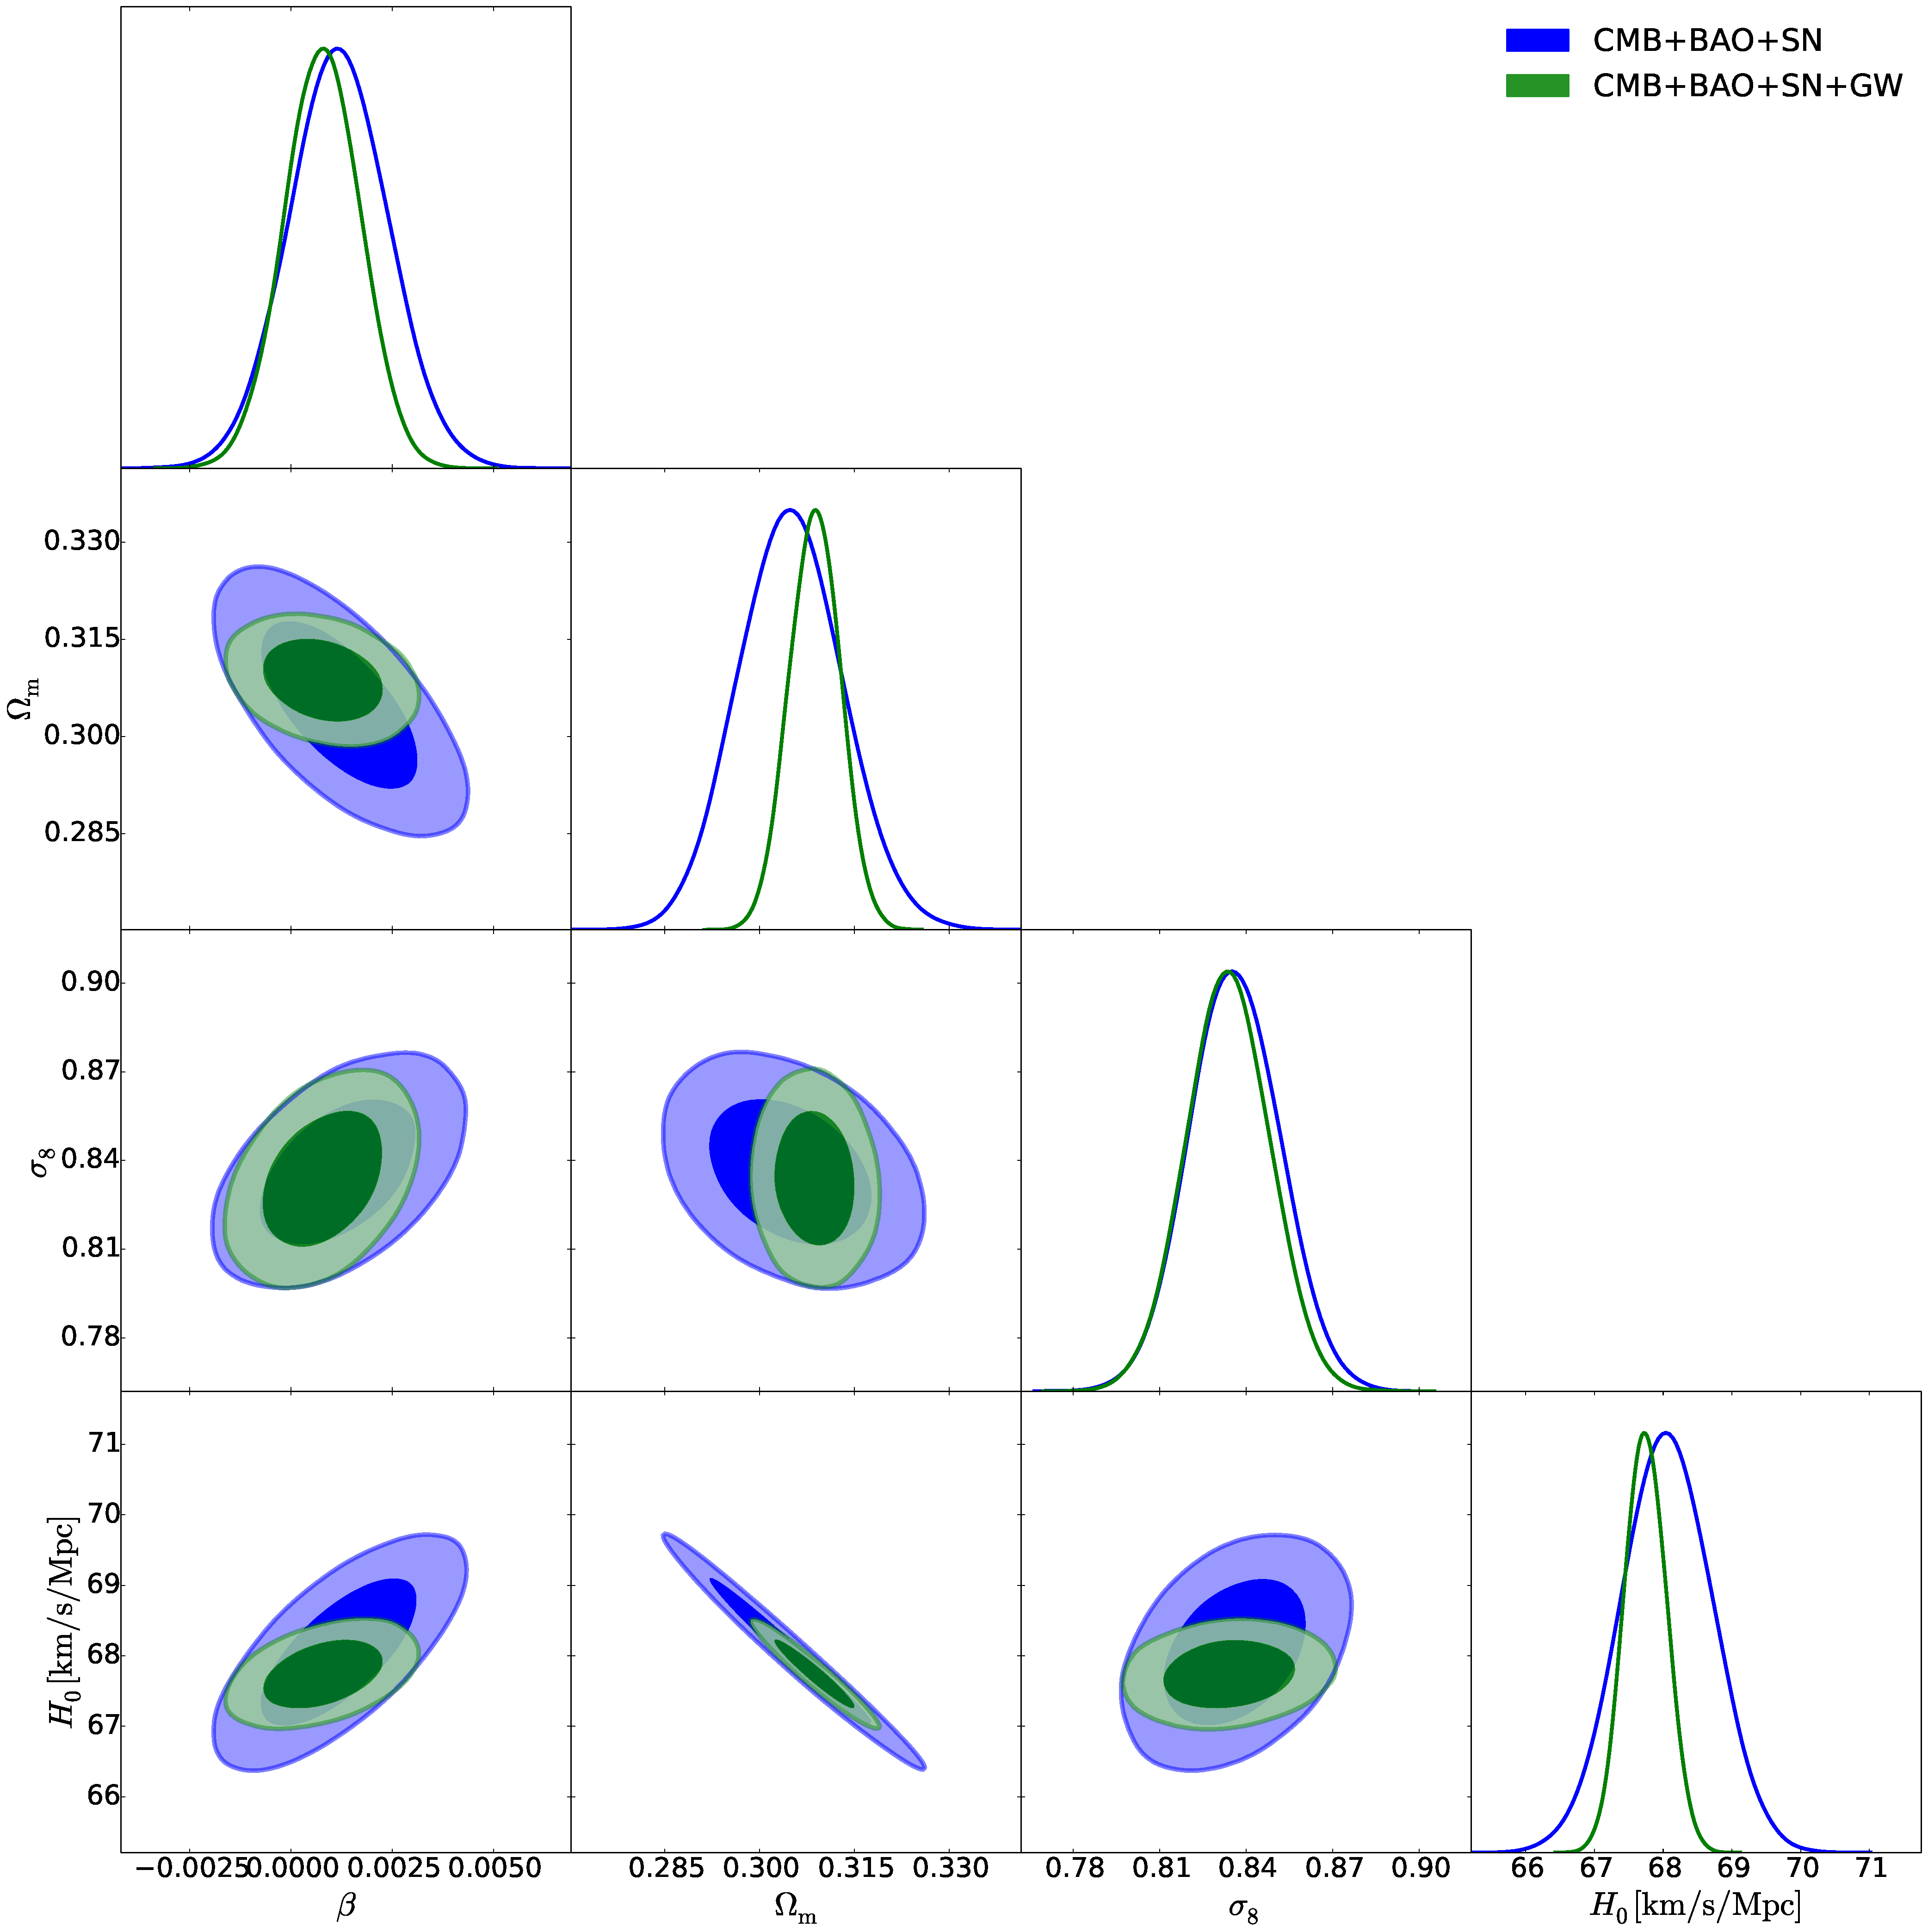
\includegraphics[scale=0.19]{ilcdmhpc.pdf}

\centering \caption{\label{fig1} Observational constraints (68.3\% and 95.4\% confidence level) on the I$\Lambda$CDM1 model with $Q=\beta H \rho_{\rm c}$ by using the CMB+BAO+SN and CMB+BAO+SN+GW data.}
\end{figure*}
%%%%%%%%%%%%%%%%%%%%%%%%%%%%%%%%%%%%%%%
%%%%%%%%%%%%%%%%%%%%%%%%%%%%%%%%%%%%%%%%%%%%%
%%%%%fig1
\begin{figure*}[!htp]
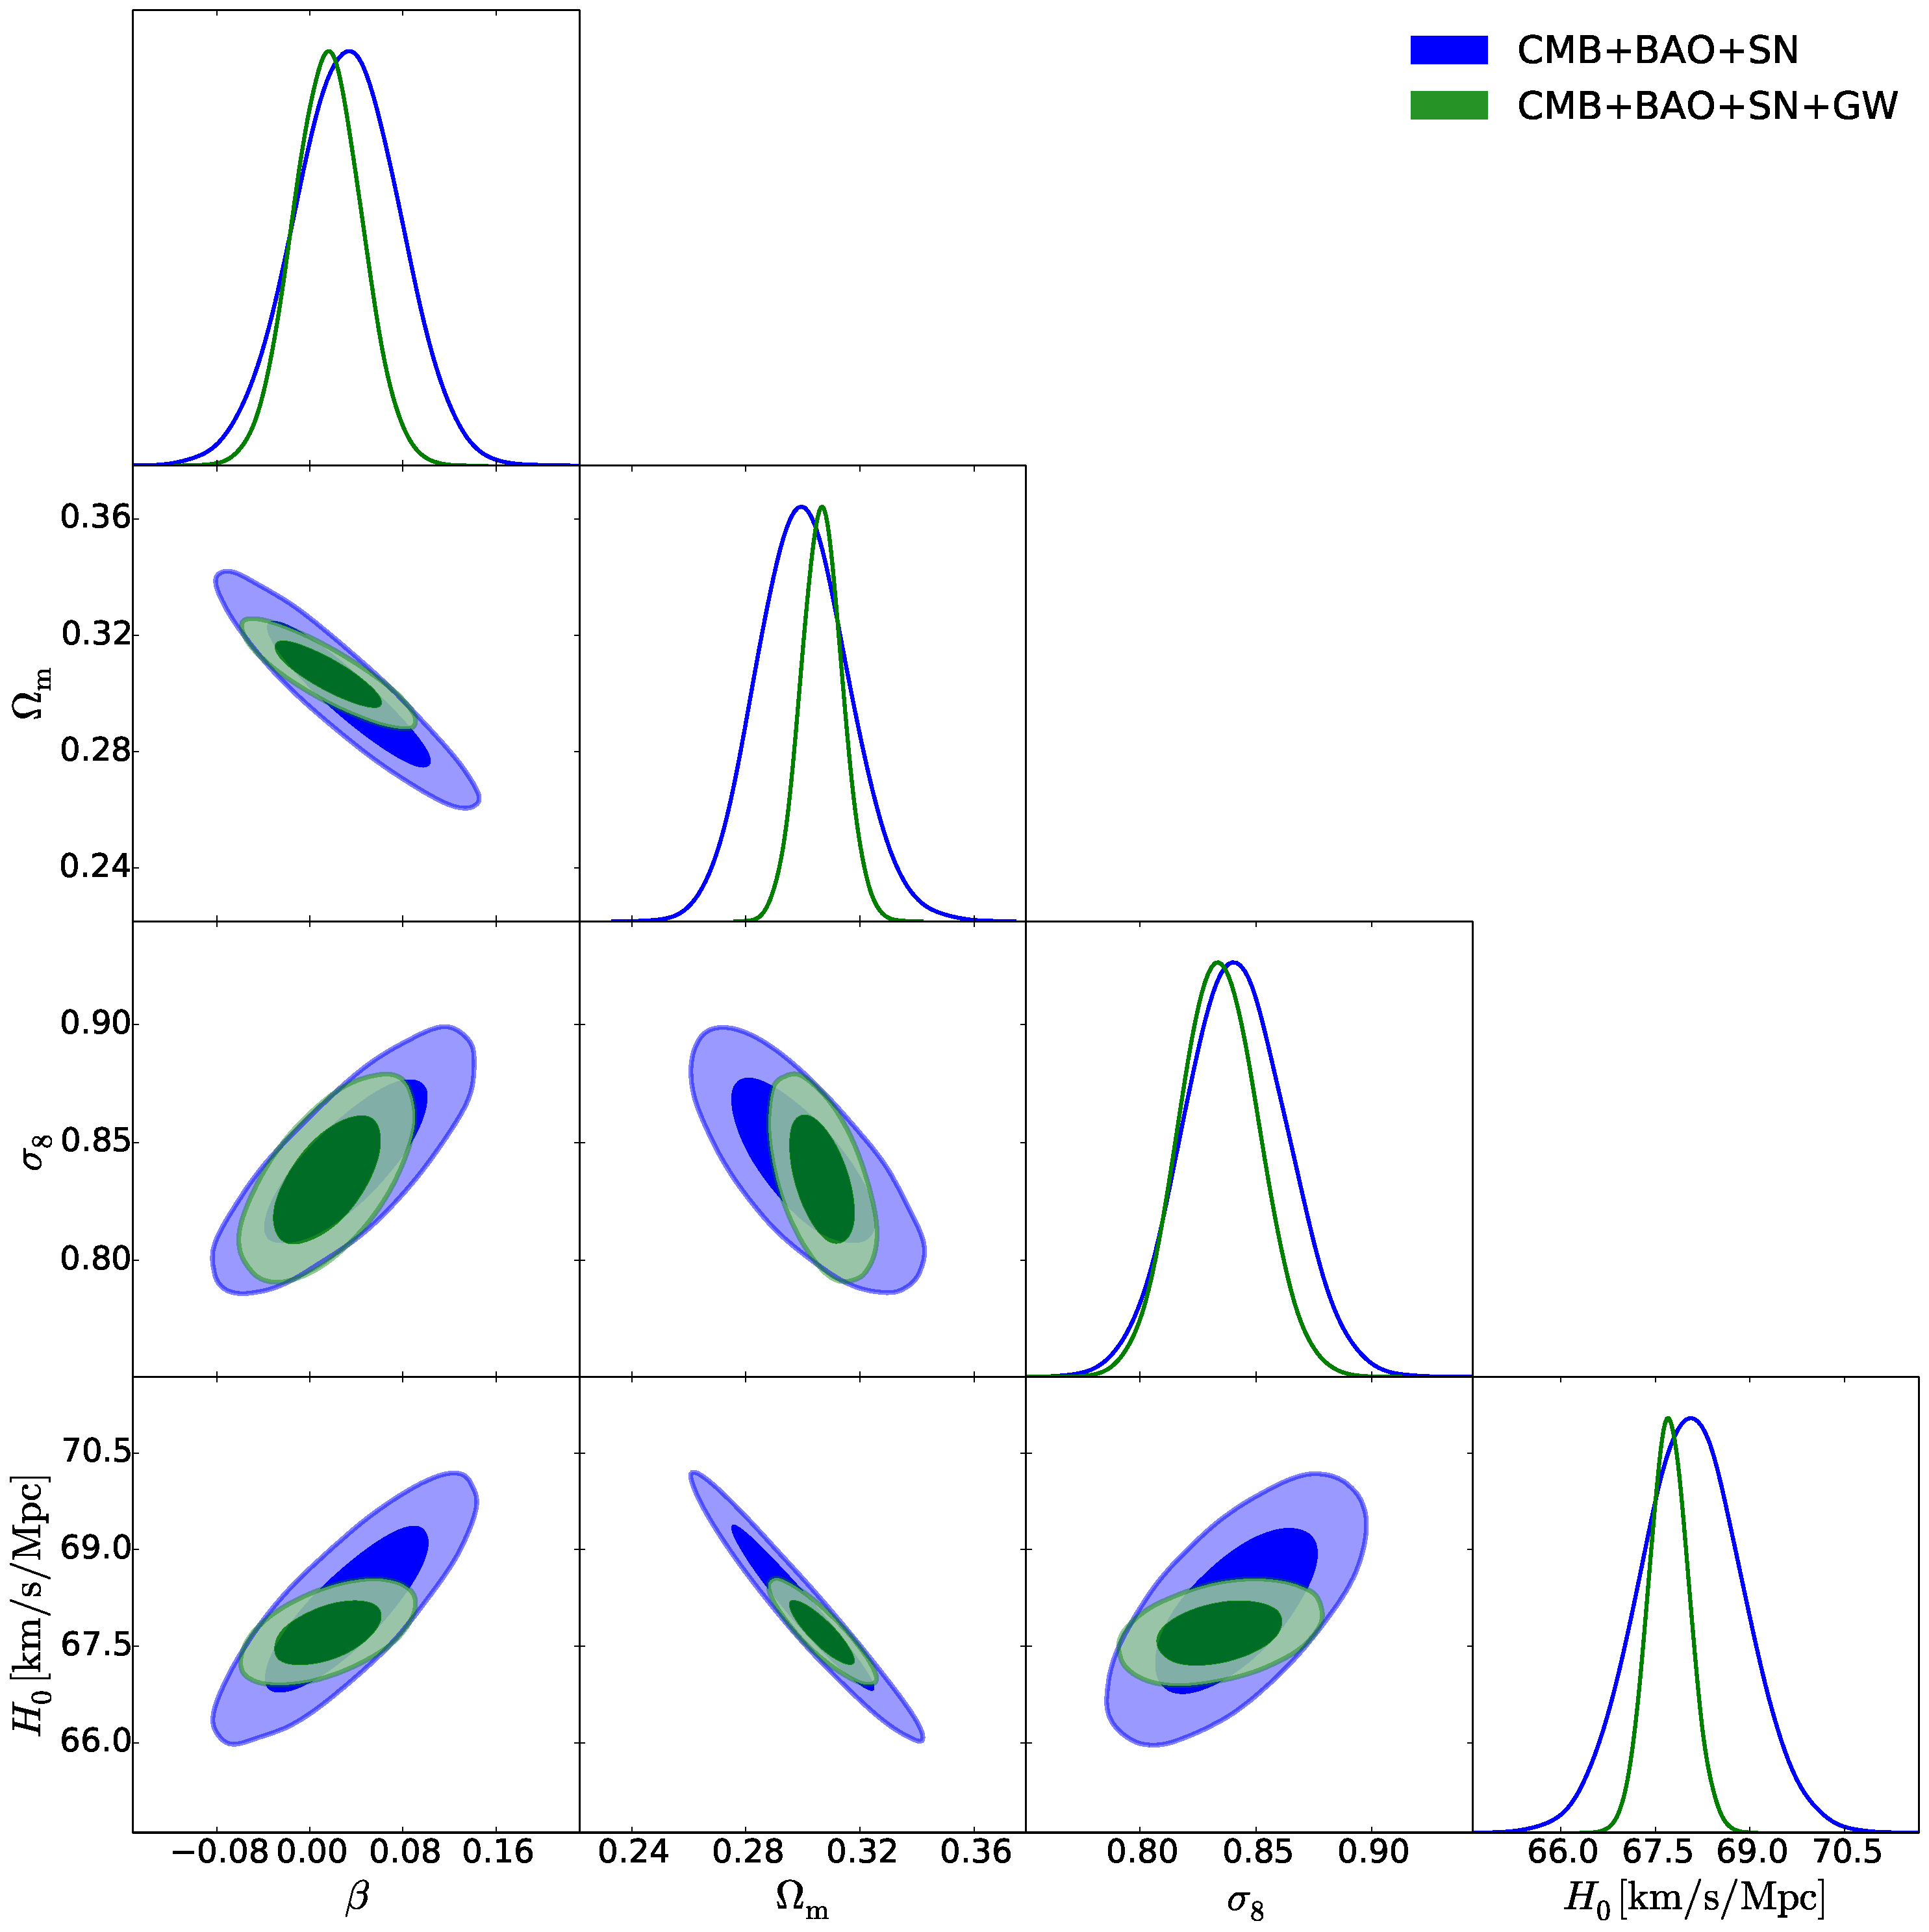
\includegraphics[scale=0.25]{ilcdmh0pc.pdf}

\centering \caption{\label{fig2} Observational constraints (68.3\% and 95.4\% confidence level) on the I$\Lambda$CDM2 model with $Q=\beta H_{0} \rho_{\rm c}$ by using the CMB+BAO+SN and CMB+BAO+SN+GW data.}
\end{figure*}
%%%%%%%%%%%%%%%%%%%%%%%%%%%%%%%%%%%%%%%
%%%%%%%%%%%%%%%%%%%%%%%%%%%%%%%%%%%%%%%%%%%%%
%%%%%fig1
\begin{figure*}[!htp]
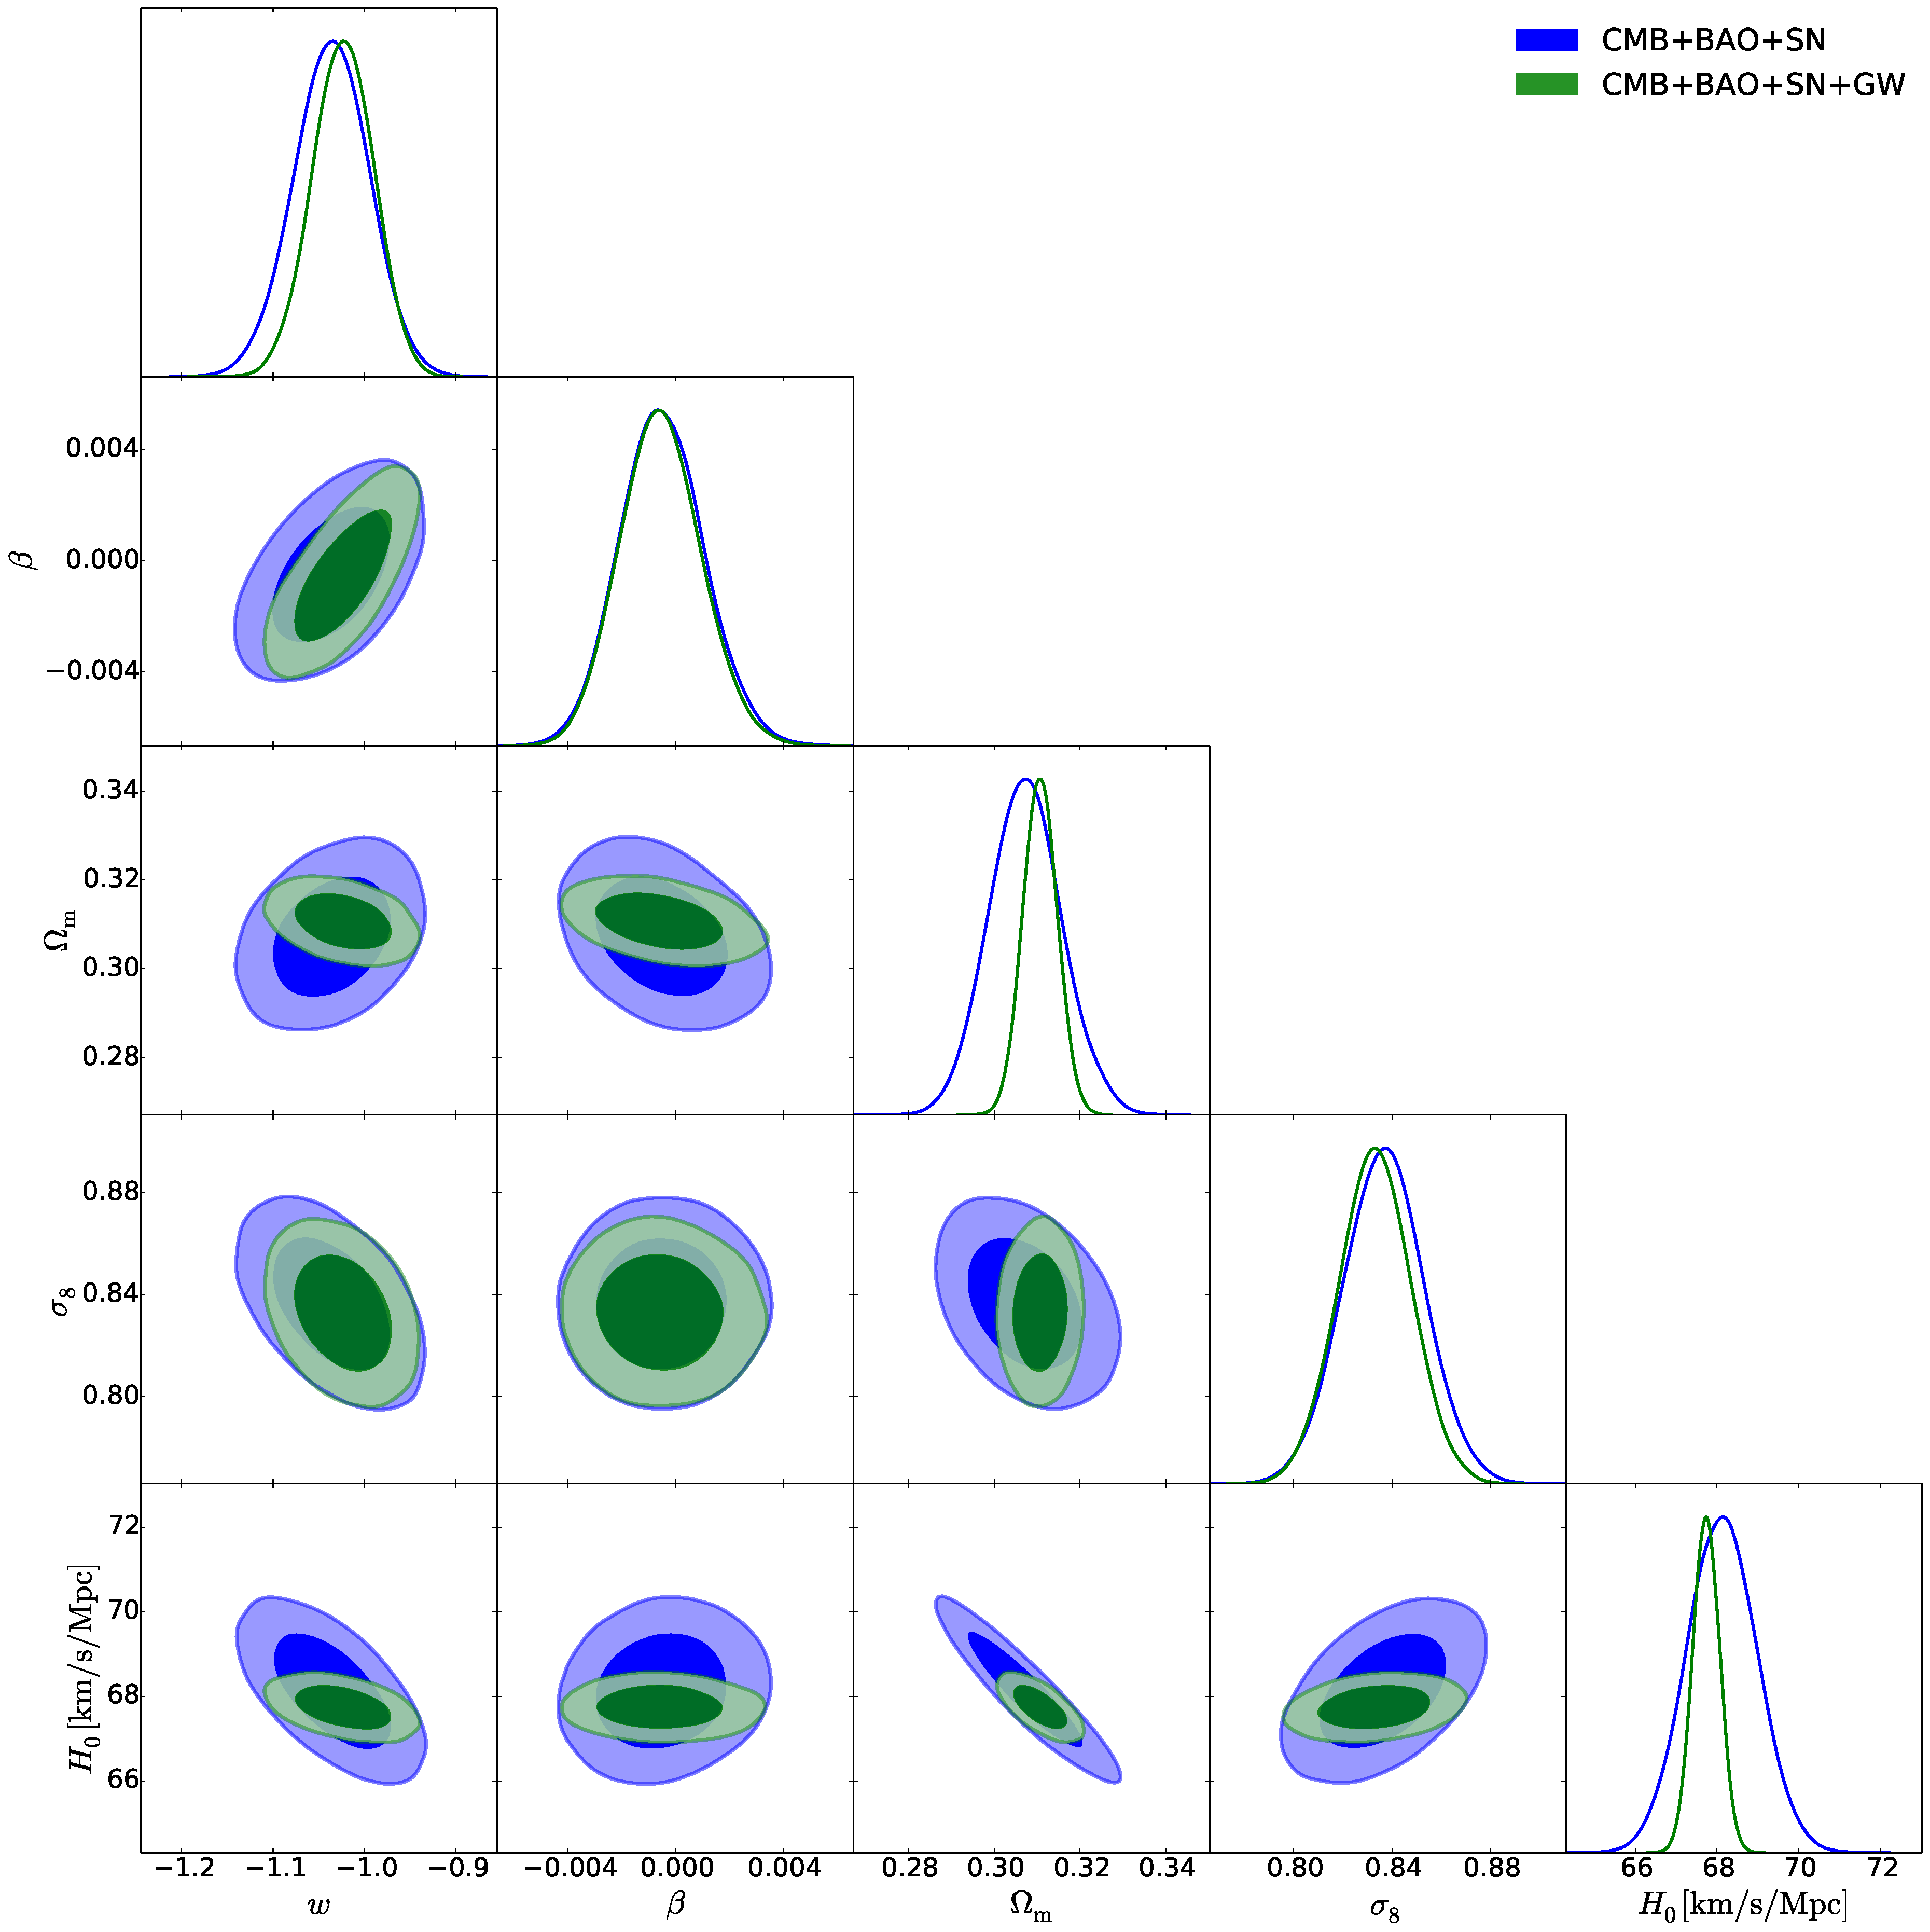
\includegraphics[scale=0.25]{iwcdmhpc.pdf}

\centering \caption{\label{fig3} Observational constraints (68.3\% and 95.4\% confidence level) on the I$w$CDM1 model with $Q=\beta H \rho_{\rm c}$ by using the CMB+BAO+SN and CMB+BAO+SN+GW data.}
\end{figure*}

\begin{figure*}[!htp]
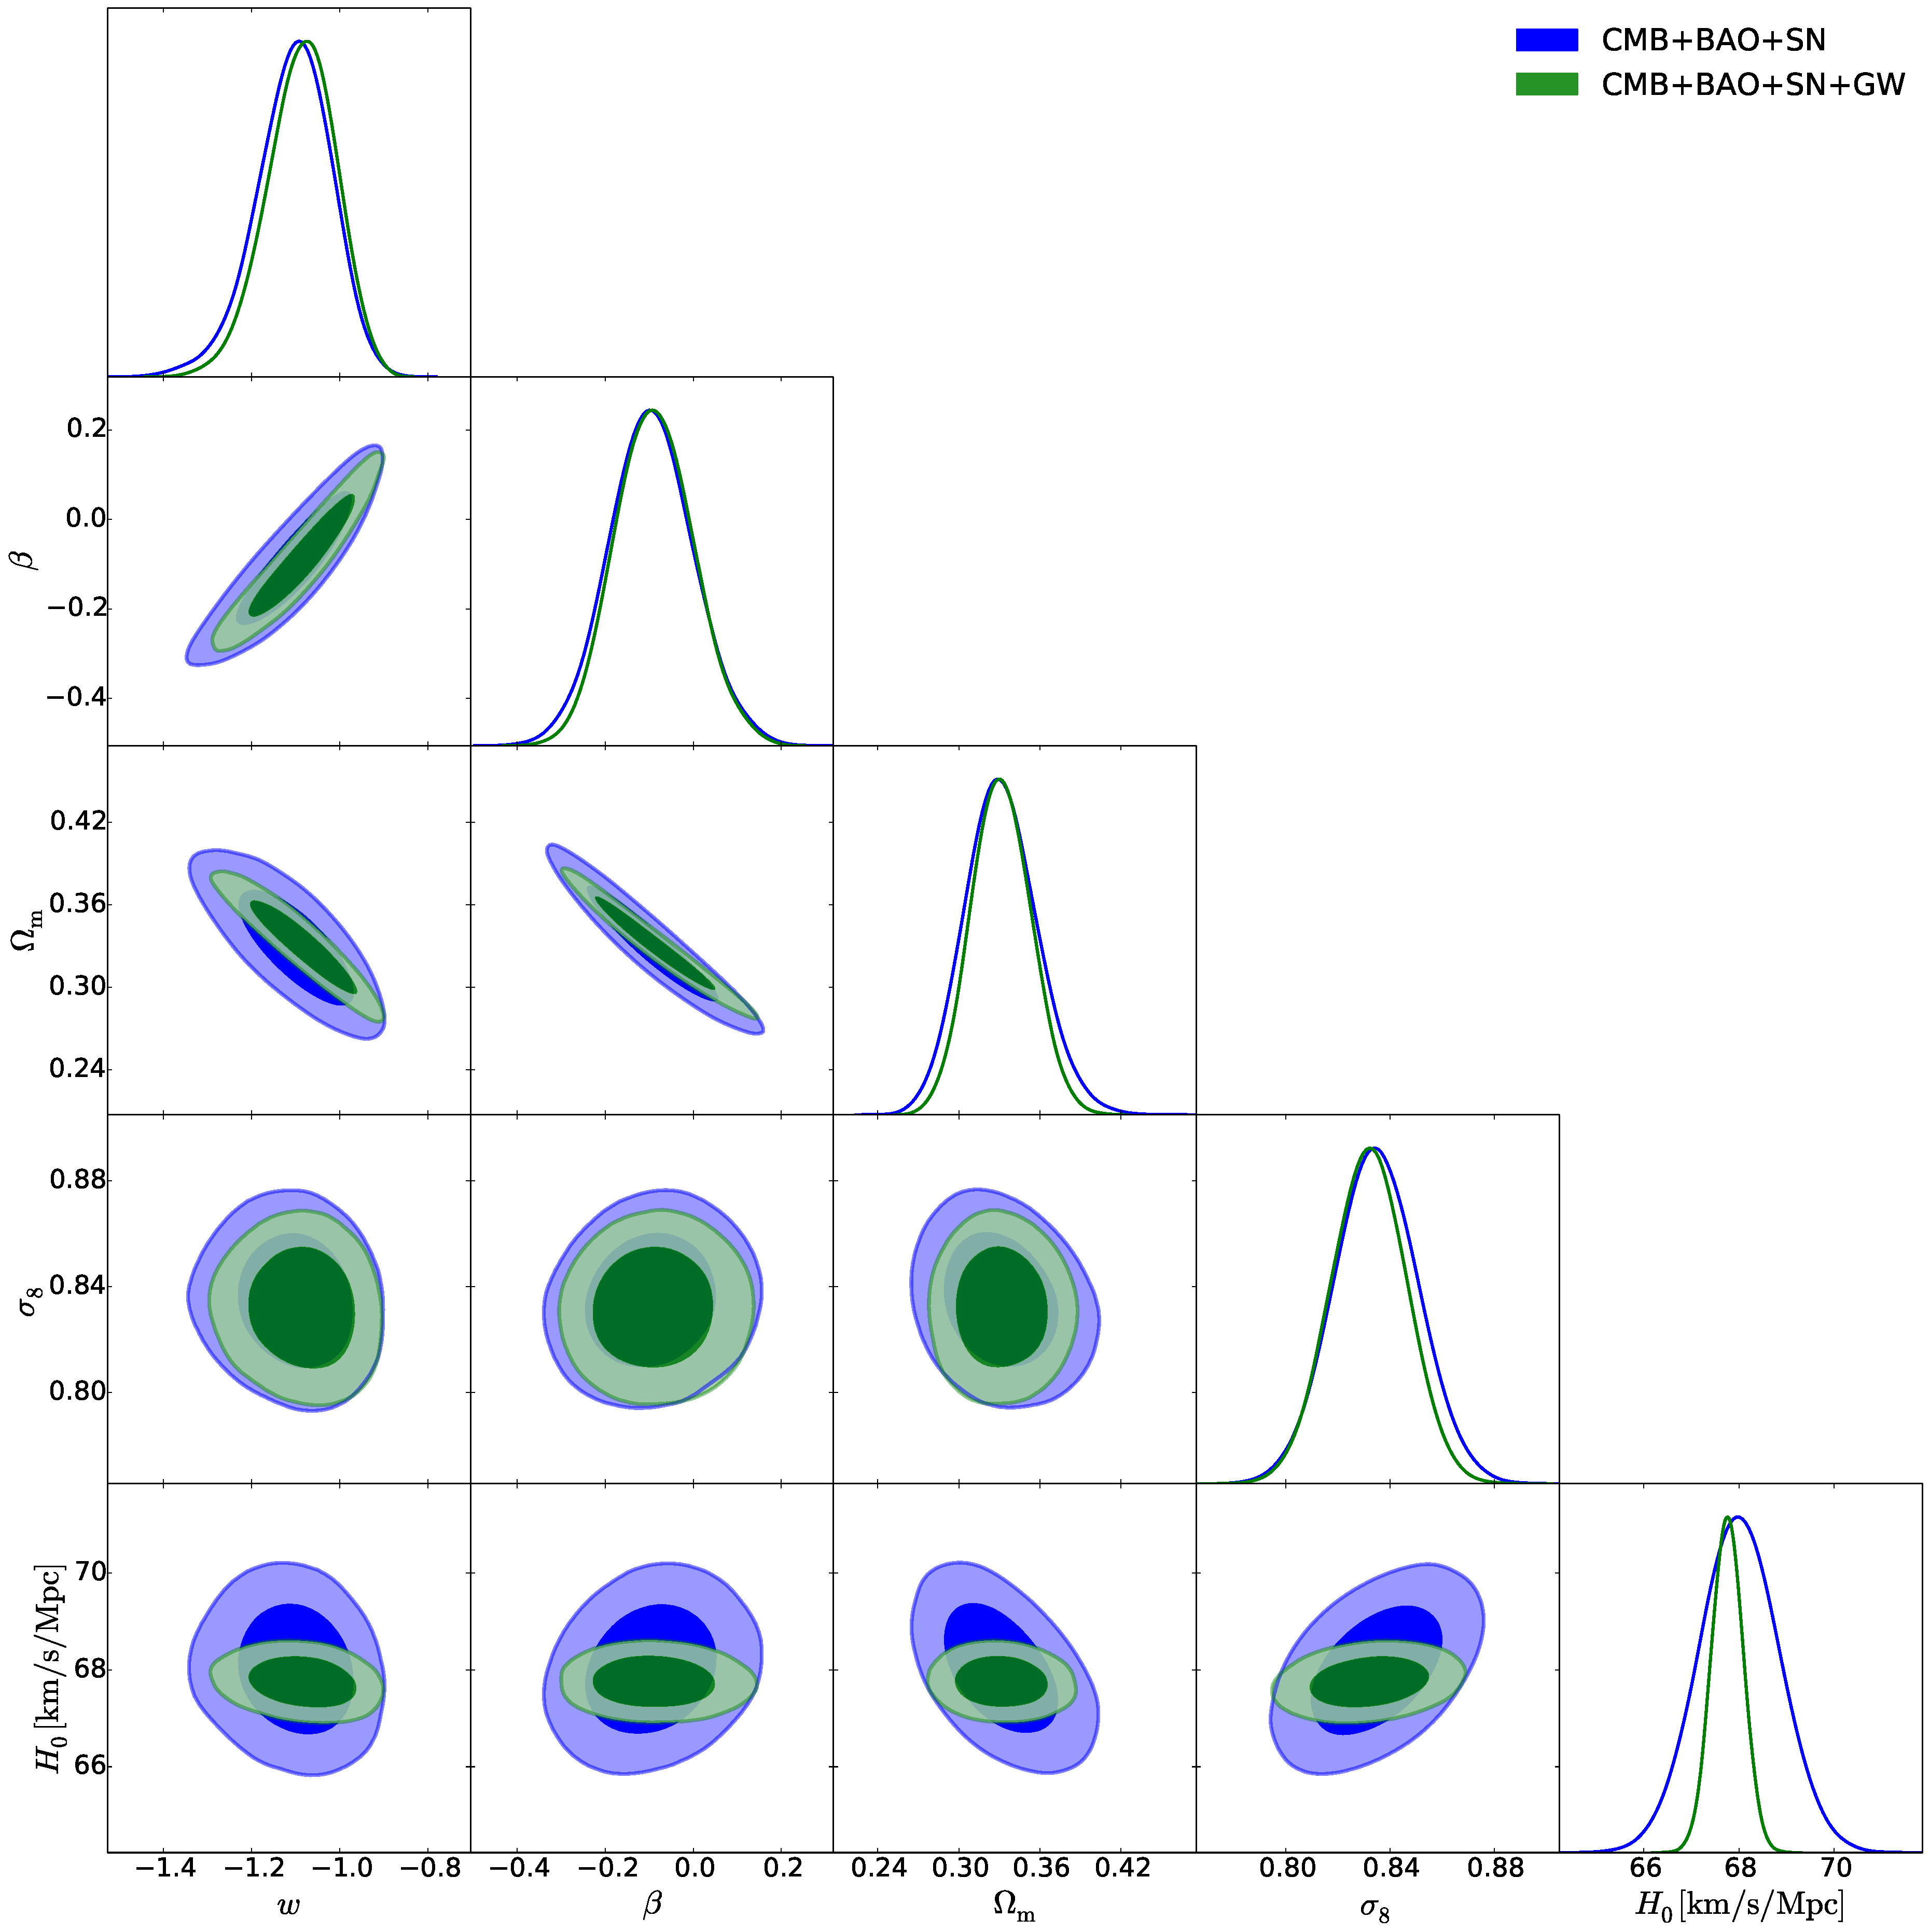
\includegraphics[scale=0.25]{iwcdmh0pc.pdf}

\centering \caption{\label{fig4} Observational constraints (68.3\% and 95.4\% confidence level) on the I$w$CDM2 model with $Q=\beta H_{0} \rho_{\rm c}$ by using the CMB+BAO+SN and CMB+BAO+SN+GW data.}
\end{figure*}
%%%%%%%%%%%%%%%%%%%%%%%%%%%%%%%%%%%%%%%
%%%%%%%%%%%%%%%%%%%%%%%%%%%%%%%%%%%%%%%%%%%%%


%%%%%%%%%%%%%%%%%%%%%%%%%%%%%%%%%%%%%%%
%%%%%%%%%%%%%%%table1%%%%%%%%%%%%%%%%%%%%%%%%

\begin{table*}\small
\setlength\tabcolsep{2pt}
\renewcommand{\arraystretch}{1.5}
\centering
\caption{\label{tab1}Fitting results (68.3\% confidence level) for the I$\Lambda$CDM models using CBS and CBS+GW. Here, CBS stands for CMB+BAO+SN.}
\begin{tabular}{ccccccccc}


\hline Model &\multicolumn{2}{c}{I$\Lambda$CDM1 ($Q=\beta H\rho_{\rm c}$)}&&\multicolumn{2}{c}{I$\Lambda$CDM2 ($Q=\beta H_{0}\rho_{\rm c}$)}\\
           \cline{2-3}\cline{5-6}
       Data  & CBS&CBS+GW &&CBS&CBS+GW \\

\hline
$\Omega_{\rm m}$                         &$0.305^{+0.008}_{-0.0081}$
                                         &$0.3088^{+0.0039}_{-0.004}$
                                         &&$0.3^{+0.015}_{-0.017}$
                                         &$0.3066\pm0.0071$
                                         \\

$H_0\,[{\rm km}/{\rm s}/{\rm Mpc}]$      &$68.05^{+0.65}_{-0.64}$
                                         &$67.74\pm0.3$
                                         &&$68.06\pm0.8$
                                         &$67.71\pm0.31$
                                         \\

$\beta$                                  &$0.0012\pm0.0012$
                                         &$0.00078^{+0.00092}_{-0.00091}$
                                         &&$0.031\pm0.044$
                                         &$0.015\pm0.029$
                                         \\

$\sigma_{8}$                             &$0.836\pm0.015$
                                         &$0.834\pm0.014$
                                         &&$0.841\pm0.022$
                                         &$0.834\pm0.017$
                                         \\



\hline
\end{tabular}

\end{table*}
%%%%%%%%%%%%%%%%%%%%%%%%%%%%%%%%%%%%%
\begin{table*}\small
\setlength\tabcolsep{2pt}
\renewcommand{\arraystretch}{1.5}
\centering
\caption{\label{tab2}Fitting results (68.3\% confidence level) for the I$w$CDM model using CBS and CBS+GW. Here, CBS stands for CMB+BAO+SN.}
\begin{tabular}{ccccccccc}


\hline Model &\multicolumn{2}{c}{I$w$CDM1 ($Q=\beta H\rho_{\rm c}$)}&&\multicolumn{2}{c}{I$w$CDM2 ($Q=\beta H_{0}\rho_{\rm c}$)}\\
           \cline{2-3}\cline{5-6}
       Data  & CBS&CBS+GW &&CBS&CBS+GW\\

\hline
$\Omega_{\rm m}$                         &$0.3073^{+0.0081}_{-0.0082}$
                                         &$ 0.3107\pm0.0039$
                                         &&$0.332^{+0.025}_{-0.028}$
                                         &$0.331\pm0.022$\\

$H_0\,[{\rm km}/{\rm s}/{\rm Mpc}]$      &$68.13^{+0.84}_{-0.83}$
                                         &$67.74\pm0.32$
                                         &&$68\pm0.82$
                                         &$67.76^{+0.32}_{-0.33}$\\

$\beta$                                  &$-0.0005\pm0.0015$
                                         &$-0.0005\pm0.0015$
                                         &&$-0.095\pm0.093$
                                         &$-0.088\pm0.087$\\

$\sigma_{8}$                             &$0.837\pm0.016$
                                         &$0.833\pm0.014$
                                         &&$0.835\pm0.016$
                                         &$0.832\pm0.014$\\

$w$                                      &$-1.036\pm0.04$
                                         &$-1.024\pm0.033$
                                         &&$-1.105^{+0.093}_{-0.075}$
                                         &$-1.087^{+0.086}_{-0.071}$\\


\hline
\end{tabular}

\end{table*}
%%%%%%%%%%%%%%%table2%%%%%%%%%%%%%%%%%%%%%%%%
\begin{table*}\small
\setlength\tabcolsep{2pt}
\renewcommand{\arraystretch}{1.5}
\centering
\caption{\label{tab3}Constraint errors for cosmological parameters of the I$\Lambda$CDM models and the I$w$CDM models using CBS and CBS+GW. Here, CBS stands for CMB+BAO+SN.}
\begin{tabular}{ccccccccccc}


\hline Model &\multicolumn{2}{c}{I$\Lambda$CDM1 ($Q=\beta H\rho_{\rm c}$)}&\multicolumn{2}{c}{I$\Lambda$CDM2 ($Q=\beta H_{0}\rho_{\rm c}$)}&&\multicolumn{2}{c}{I$w$CDM1 ($Q=\beta H\rho_{\rm c}$)}&\multicolumn{2}{c}{I$w$CDM2 ($Q=\beta H_{0}\rho_{\rm c}$)}\\
           \cline{2-5}\cline{7-10}
       Data  & CBS&CBS+GW &CBS&CBS+GW &&CBS&CBS+GW&CBS&CBS+GW\\

\hline
$\sigma(\Omega_{\rm m})$                         &$0.0081$
                                         &$0.0040$
                                         &$0.0160$
                                         &$0.0071$
                                         &&$0.0082$
                                         &$0.0039$
                                         &$0.0265$
                                         &$0.022$\\

$\sigma(H_0\,[{\rm km}/{\rm s}/{\rm Mpc}])$      &$0.6450$
                                         &$0.3$
                                         &$0.8$
                                         &$0.31$
                                         &&$0.8350$
                                         &$0.32$
                                         &$0.82$
                                         &$0.3250$\\

$\sigma(\beta)$                                  &$0.0012$
                                         &$0.000915$
                                         &$0.044$
                                         &$0.029$
                                         &&$0.0015$
                                         &$0.0015$
                                         &$0.093$
                                         &$0.087$\\

$\sigma(\sigma_{8})$                             &$0.015$
                                         &$0.014$
                                         &$0.022$
                                         &$0.017$
                                         &&$0.016$
                                         &$0.014$
                                         &$0.016$
                                         &$0.014$\\

$\sigma(w)$                                      &$-$
                                         &$-$
                                         &$-$
                                         &$-$
                                         &&$0.04$
                                         &$0.033$
                                         &$0.0845$
                                         &$0.0789$\\


\hline
\end{tabular}

\end{table*}
%%%%%%%%%%%%%%%%%%%%%%%%%%%%%%%%%%%%%%%%%%%%
\begin{table*}\small
\setlength\tabcolsep{2pt}
\renewcommand{\arraystretch}{1.5}
\centering
\caption{\label{tab4}Constraint accuracies for cosmological parameters of the I$\Lambda$CDM models and the I$w$CDM models using CBS, and CBS+GW. Here, CBS stands for CMB+BAO+SN.}
\begin{tabular}{ccccccccccc}


\hline Model &\multicolumn{2}{c}{I$\Lambda$CDM1 ($Q=\beta H\rho_{\rm c}$)}&\multicolumn{2}{c}{I$\Lambda$CDM2 ($Q=\beta H_{0}\rho_{\rm c}$)}&&\multicolumn{2}{c}{I$w$CDM1 ($Q=\beta H\rho_{\rm c}$)}&\multicolumn{2}{c}{I$w$CDM2 ($Q=\beta H_{0}\rho_{\rm c}$)}\\
           \cline{2-5}\cline{7-10}
       Data  & CBS&CBS+GW &CBS&CBS+GW &&CBS&CBS+GW&CBS&CBS+GW\\

\hline
$\varepsilon(\Omega_{\rm m})$                         &$0.0266$
                                         &$0.0130$
                                         &$0.0533$
                                         &$0.0232$
                                         &&$0.0267$
                                         &$0.0126$
                                         &$0.0798$
                                         &$0.0665$\\

$\varepsilon(H_0\,[{\rm km}/{\rm s}/{\rm Mpc}])$      &$0.0095$
                                         &$0.0044$
                                         &$0.0118$
                                         &$0.0045$
                                         &&$0.0123$
                                         &$0.0047$
                                         &$0.0121$
                                         &$0.0048$\\

$\varepsilon(\beta)$                                  &$1$
                                         &$1.1731$
                                         &$1.4194$
                                         &$1.9333$
                                         &&$3$
                                         &$3$
                                         &$0.9789$
                                         &$0.9886$\\

$\varepsilon(\sigma_{8})$                             &$0.0179$
                                         &$0.0168$
                                         &$0.0261$
                                         &$0.0204$
                                         &&$0.0191$
                                         &$0.0168$
                                         &$0.0192$
                                         &$0.0168$\\

$\varepsilon(w)$                                      &$-$
                                         &$-$
                                         &$-$
                                         &$-$
                                         &&$0.0386$
                                         &$0.0322$
                                         &$0.0765$
                                         &$0.0726$\\


\hline
\end{tabular}

\end{table*}
%%%%%%%%%%%%%%%%%


\section{Results and discussion}\label{sec4}

In this section, we exhibit the main constraint results in Figs.~\ref{fig1}--\ref{fig4}, and summarize in Tables~\ref{tab1}--\ref{tab4}. In Figs.~\ref{fig1}--\ref{fig4}, the constraint results for the I$\Lambda$CDM1 model with $Q=\beta H\rho_{\rm c}$, I$\Lambda$CDM2 model with $Q=\beta H_{0}\rho_{\rm c}$, and I$w$CDM1 model with $Q=\beta H\rho_{\rm c}$, I$w$CDM2 model with $Q=\beta H_{0}\rho_{\rm c}$ are shown, respectively. In these figures, one-dimensional marginalized posterior distributions and the two-dimensional contours (68.3\% and 95.4\% confidence level) from CMB+BAO+SN and CMB+BAO+SN+GW are colored by blue and green, respectively. The fit values of the cosmological parameters for the IDE models are given in Tables \ref{tab1} and \ref{tab2}. The constraint errors of the cosmological parameters are given in Tables \ref{tab3}, and the constraint accuracies are given in Tables \ref{tab4}. Here, the error $\sigma$ is the root-mean-square of $\sigma_+$ and $\sigma_-$, and for a parameter $\xi$ the accuracy $\varepsilon(\xi)$ can be defined as $\varepsilon(\xi)=\sigma(\xi)/\xi$. For convenience, the data combination ``CMB+BAO+SN" is abbreviated as ``CBS" in the following.


At first glance in these figures, we can easily find that the addition of GW standard sirens data can tighten the constraint on $H_0$ and $\Omega_{\rm m}$ significantly (except this case in the I$w$CDM2 model with $Q=\beta H_{0}\rho_{\rm c}$, which will be discussed in the following), but for the other parameters, the constraints are slightly weak.


The constraint results for the I$\Lambda$CDM1 model with $Q=\beta H\rho_{\rm c}$ are shown in Fig.~\ref{fig1}. We find that the CBS data provided a 0.95\% measurement for $H_0$, whereas the combined CBS+GW data provided a 0.44\% measurement. For the parameter $\Omega_{\rm m}$, the CBS data can give a constraint accuracy at 2.66\%. When adding the GW data, the constraint accuracy on $\Omega_{\rm m}$ can be improved to 1.3\% level with the CBS+GW data. Obviously, both of these two parameters can be constrained more stringent with the help of GW data. \red{Note here that, since central value of the coupling constant $\beta$ in IDE models is around zero, the relative error for this parameter will be immensely influenced by the statistic fluctuations. Therefore, the absolute error is more reliable for quantifying the improvement of this parameter. The addition of the GW data will tighten the constraint on the coupling constant $\beta$, with the absolute error improved from $\sigma(\beta)=1.2 \times 10^{-3}$ to $\sigma(\beta)=9.15 \times 10^{-4}$.}


The constraint results for the I$\Lambda$CDM2 model with $Q=\beta H_{0}\rho_{\rm c}$ are shown in Fig.~\ref{fig2}. For this model, the CBS data can provide a 1.18\% measurement for $H_0$,  while the CBS+GW data can measure $H_0$ at the 0.45\% level. With respect to the parameter $\Omega_{\rm m}$, the CBS+GW data can give a constraint accuracy on $\Omega_{\rm m}$ at 2.32\%, better than the constraint from CBS data with just a 5.33\% accuracy. \red{For the coupling constant $\beta$, the result is similar to the case of I$\Lambda$CDM1 model, and the constraint error could be improved  from $\sigma(\beta)=4.4 \times 10^{-2}$ to $\sigma(\beta)=2.9 \times 10^{-2}$ with the addition of GW data.}

The results for the I$w$CDM1 model with $Q=\beta H\rho_{\rm c}$ are shown in Fig.~\ref{fig3}. From this figure, we find the situation is similar to that of the I$\Lambda$CDM models. We can see that the CBS data can only provide a 1.23\% measurement for $H_0$, while the combined CBS+GW data constrain the $H_0$ with a 0.47\% accuracy. As for the measurement of $\Omega_{\rm m}$, we find that the constraint result of the CBS+GW data is also better than the CBS data. When adding the GW data, the constraint accuracy of $\Omega_{\rm m}$ will be improved from 2.67\% to 1.26\%. For the parameter $w$, there is a slight improvement when adding the GW data, with the accuracy enhanced from 3.86\% to 3.22\%. \red{For coupling parameter $\beta$, the constraint error is at the $\sigma(\beta)=1.5 \times 10^{-3}$ level in both of the data combinations. The improvement in this case is not evident.}

Finally, we will investigate the I$w$CDM2 model with $Q=\beta H_{0}\rho_{\rm c}$, of which the constraint results are shown in Fig.~\ref{fig4}. Totally speaking, we find that the constraint accuracy on $\Omega_{\rm m}$ is pretty worse compared with the cases in the above mentioned three models. When adding the GW data, the constraint on $\Omega_{\rm m}$ is at the 6.65\% level by the combined CBS+GW data, slightly better than the CBS data with a 7.98\% accuracy. In addition, we also find that the CBS data can provide a 1.21\% measurement for $H_0$, and the combined CBS+GW data provides a 0.48\% measurement for $H_0$. Similar to the case of I$w$CDM1 model with $Q=\beta H\rho_{\rm c}$, the accuracy of $w$ only has a slight improvement, which is from 7.65\% to 7.26\%. \red{For the coupling parameter $\beta$, when we adding the GW data, the constraint error would slightly decreased, from $\sigma(\beta)=9.3 \times 10^{-2}$ to $\sigma(\beta)=8.7 \times 10^{-2}$.}

In summary, for all the IDE models considered in this paper, the future GW standard siren data observed by the ET can indeed improve the constraint accuracies on most of the cosmological parameters, e.g., $\Omega_{\rm m}$, $H_0$, and $w$. \red{Additionally, for the coupling constant $\beta$, when adding the GW data, the constraint error would also be reduced, except for the case in I$w$CDM1 model.}



%%%%%%%%%%%%%%%table%%%%%%%%%%%%%%%%%%%%%%%%
\section{Conclusion}\label{sec5}

In this paper, we have investigated                                                                                                                                                                                                                                                                                                                                                                                                                                                                                                                                                                                                                                                                                                                                                                                                                                                                                                                                                                                                                                                                                                                                                                                                                                                                                                                                                                                                                                                                                                                                                                                                                                                                                                                                                                                                                                                                                                                                                                                                                                                                                                                                                                                                                                                   how the GW standard sirens impact the parameter estimation for the IDE models. We consider four various IDE models, i.e., the I$\Lambda$CDM1 ($Q=\beta H\rho_{\rm c}$) model, I$\Lambda$CDM2 ($Q=\beta H_{0}\rho_{\rm c}$) model, I$w$CDM1 ($Q=\beta H_{0}\rho_{\rm c}$) model, and I$w$CDM2 ($Q=\beta H_{0}\rho_{\rm c}$) respectively. The conventional optical observational data we used in this paper include, the Planck 2015 CMB data, the BAO measurements, and the SN data of Pantheon compilation. For the GW data, we simulated 1000 GW events based on the ET's ten-years observation. In order to quantify the constraint ability of the additional GW data, we consider two cases of data combination, namely CBS and CBS+GW, to constrain these models.

We find that the future GW standard sirens can significantly improve the constraints on most of the cosmological parameters for all the IDE models. When adding the GW standard siren data, the constraint accuracy of $H_0$ can be remarkably improved, from 0.95\%, 1.18\%, 1.23\%, 1.21\% to the level of 0.44\%, 0.45\%, 0.47\% and 0.48\% for the I$\Lambda$CDM1, I$\Lambda$CDM2, I$w$CDM1, and I$w$CDM2 models, respectively. Moreover, as for the parameter $\Omega_{\rm m}$, the constraint accuracy was improved from 2.66\%, 5.33\%, 2.67\%, 7.98\% to 1.30\%, 2.32\%, 1.26\% and 6.65\%, for the four considered models separately. \red{For the coupling constant $\beta$, when adding the GW data, the constraint absolute error $\sigma(\beta)$ can also be promoted, from $1.2 \times 10^{-3}$, $4.4 \times 10^{-2}$, $9.3 \times 10^{-2}$ to $9.15 \times 10^{-4}$, $2.9 \times 10^{-2}$, and $8.7 \times 10^{-2}$ for the I$\Lambda$CDM1, I$\Lambda$CDM2, and I$w$CDM2 models respectively. While, in the I$w$CDM1 model, the improvement is not conspicuous for this parameter.} For the parameter $w$ in the I$w$CDM models, the constraint accuracy could be improved as well when adding the GW data, i.e., from 3.86\% to 3.22\% for I$w$CDM1 model and from 7.65\% to 8.26\% for I$w$CDM2 model.

All in all, the precision of the parameter constraint can be promoted effectively with the consideration of future GW observation in the considered four IDE models. The results are consistent with the other extensively studied dark energy models. Thus, we can conclude that the improvement of the parameter constraint precision with future GW standard siren data may be independent of the cosmological models in the background. More DE and MG models should be explored to make this conclusion more reliable.
\begin{acknowledgments}
This work was supported by the National Natural Science Foundation of China (Grants Nos.~11875102, 11835009, 11690021, and 11522540) and the National Program for Support of Top-Notch Young Professionals.

\end{acknowledgments}



\begin{thebibliography}{99}

 %%observations
%\cite{Riess:1998cb}
\bibitem{Riess:1998cb}
  A.~G.~Riess {\it et al.} [Supernova Search Team Collaboration],
  Observational evidence from supernovae for an accelerating universe and a cosmological constant,
  Astron.\ J.\  {\bf 116} (1998) 1009
 % doi:10.1086/300499
  [astro-ph/9805201].
  %%CITATION = doi:10.1086/300499;%%

%\cite{Perlmutter:1998np}
\bibitem{Perlmutter:1998np}
  S.~Perlmutter {\it et al.} [Supernova Cosmology Project Collaboration],
  Measurements of Omega and Lambda from 42 high redshift supernovae,
  Astrophys.\ J.\  {\bf 517}, 565 (1999)
 % doi:10.1086/307221
  [astro-ph/9812133].
  %%CITATION = doi:10.1086/307221;%%



%\cite{Spergel:2003cb}          
\bibitem{Spergel:2003cb}
  D.~N.~Spergel {\it et al.} [WMAP Collaboration],
  First year Wilkinson Microwave Anisotropy Probe (WMAP) observations: Determination of cosmological parameters,
  Astrophys.\ J.\ Suppl.\  {\bf 148}, 175 (2003)
 % doi:10.1086/377226
  [astro-ph/0302209].
  %%CITATION = doi:10.1086/377226;%%

%\cite{Bennett:2003bz}
\bibitem{Bennett:2003bz}
  C.~L.~Bennett {\it et al.} [WMAP Collaboration],
  First year Wilkinson Microwave Anisotropy Probe (WMAP) observations: Preliminary maps and basic results,
  Astrophys.\ J.\ Suppl.\  {\bf 148}, 1 (2003)
 % doi:10.1086/377253
  [astro-ph/0302207].
  %%CITATION = doi:10.1086/377253;%%

%\cite{Tegmark:2003ud}
\bibitem{Tegmark:2003ud}
  M.~Tegmark {\it et al.} [SDSS Collaboration],
  Cosmological parameters from SDSS and WMAP,
  Phys.\ Rev.\ D {\bf 69}, 103501 (2004)
 % doi:10.1103/PhysRevD.69.103501
  [astro-ph/0310723].
  %%CITATION = doi:10.1103/PhysRevD.69.103501;%%

%\cite{Abazajian:2004aja}
\bibitem{Abazajian:2004aja}
  K.~Abazajian {\it et al.} [SDSS Collaboration],
  The Second data release of the Sloan digital sky survey,
  Astron.\ J.\  {\bf 128}, 502 (2004)
 % doi:10.1086/421365
  [astro-ph/0403325].
  %%CITATION = doi:10.1086/421365;%%




%\cite{Sahni:2006pa}               3
\bibitem{Sahni:2006pa}
  V.~Sahni and A.~Starobinsky,
  Reconstructing Dark Energy,
  Int.\ J.\ Mod.\ Phys.\ D {\bf 15}, 2105 (2006)
  %doi:10.1142/S0218271806009704
  [astro-ph/0610026].
  %%CITATION = doi:10.1142/S0218271806009704;%%

%\cite{Bamba:2012cp}
\bibitem{Bamba:2012cp}
  K.~Bamba, S.~Capozziello, S.~Nojiri and S.~D.~Odintsov,
  Dark energy cosmology: the equivalent description via different theoretical models and cosmography tests,
  Astrophys.\ Space Sci.\  {\bf 342}, 155 (2012)
  %doi:10.1007/s10509-012-1181-8
  [arXiv:1205.3421 [gr-qc]].
  %%CITATION = doi:10.1007/s10509-012-1181-8;%%
  %526 citations counted in INSPIRE as of 21 Jul 2016

%\cite{Weinberg:1988cp}
\bibitem{Weinberg:1988cp}
  S.~Weinberg,
  The Cosmological Constant Problem,
  Rev.\ Mod.\ Phys.\  {\bf 61}, 1 (1989).
 % doi:10.1103/RevModPhys.61.1
  %%CITATION = doi:10.1103/RevModPhys.61.1;%%

%\cite{Peebles:2002gy}
\bibitem{Peebles:2002gy}
  P.~J.~E.~Peebles and B.~Ratra,
  The Cosmological constant and dark energy,
  Rev.\ Mod.\ Phys.\  {\bf 75}, 559 (2003)
  %doi:10.1103/RevModPhys.75.559
  [astro-ph/0207347].
  %%CITATION = doi:10.1103/RevModPhys.75.559;%%
  %3071 citations counted in INSPIRE as of 15 Oct 2017

%\cite{Copeland:2006wr}
\bibitem{Copeland:2006wr}
  E.~J.~Copeland, M.~Sami and S.~Tsujikawa,
  Dynamics of dark energy,
  Int.\ J.\ Mod.\ Phys.\ D {\bf 15}, 1753 (2006)
 % doi:10.1142/S021827180600942X
  [hep-th/0603057].
  %%CITATION = doi:10.1142/S021827180600942X;%%

%\cite{Frieman:2008sn}
\bibitem{Frieman:2008sn}
  J.~Frieman, M.~Turner and D.~Huterer,
  Dark Energy and the Accelerating Universe,
  Ann.\ Rev.\ Astron.\ Astrophys.\  {\bf 46}, 385 (2008)
 % doi:10.1146/annurev.astro.46.060407.145243
  [arXiv:0803.0982 [astro-ph]].
  %%CITATION = doi:10.1146/annurev.astro.46.060407.145243;%%
  %762 citations counted in INSPIRE as of 21 Jul 2016

%\cite{Sahni:2008zz}
\bibitem{Sahni:2008zz}
  V.~Sahni,
  Reconstructing the properties of dark energy,
  Prog.\ Theor.\ Phys.\ Suppl.\  {\bf 172}, 110 (2008).
  doi:10.1143/PTPS.172.110
  %%CITATION = doi:10.1143/PTPS.172.110;%%
  %2 citations counted in INSPIRE as of 15 Oct 2017

%\cite{Li:2011sd}
\bibitem{Li:2011sd}
  M.~Li, X.~D.~Li, S.~Wang and Y.~Wang,
  Dark Energy,
  Commun.\ Theor.\ Phys.\  {\bf 56}, 525 (2011)
  %doi:10.1088/0253-6102/56/3/24
  [arXiv:1103.5870 [astro-ph.CO]].
  %%CITATION = doi:10.1088/0253-6102/56/3/24;%%

%\cite{Kamionkowski:2007wv}
\bibitem{Kamionkowski:2007wv}
  M.~Kamionkowski,
  Dark Matter and Dark Energy,
  arXiv:0706.2986 [astro-ph].
  %%CITATION = ARXIV:0706.2986;%%
  %47 citations counted in INSPIRE as of 15 Oct 2017





%\cite{Ade:2015xua}       4
\bibitem{Ade:2015xua}
  P.~A.~R.~Ade {\it et al.} [Planck Collaboration],
  Planck 2015 results. XIII. Cosmological parameters,
  Astron.\ Astrophys.\  {\bf 594}, A13 (2016)
  %doi:10.1051/0004-6361/201525830
  [arXiv:1502.01589 [astro-ph.CO]].
  %%CITATION = doi:10.1051/0004-6361/201525830;%%
  %4229 citations counted in INSPIRE as of 19 Oct 2017



%\cite{Sahni:1999gb}           5
\bibitem{Sahni:1999gb}
  V.~Sahni and A.~A.~Starobinsky,
  The Case for a positive cosmological Lambda term,
  Int.\ J.\ Mod.\ Phys.\ D {\bf 9}, 373 (2000)
 % doi:10.1142/S0218271800000542
  [astro-ph/9904398].
  %%CITATION = doi:10.1142/S0218271800000542;%%

%\cite{Bean:2005ru}
\bibitem{Bean:2005ru}
  R.~Bean, S.~M.~Carroll and M.~Trodden,
  Insights into dark energy: interplay between theory and observation,
  astro-ph/0510059.
  %%CITATION = ASTRO-PH/0510059;%%
\bibitem{Amendola:1999er}
  L.~Amendola,
  Coupled quintessence,
  Phys.\ Rev.\ D {\bf 62}, 043511 (2000)
  %doi:10.1103/PhysRevD.62.043511
[astro-ph/9908023].

\bibitem{Amendola:1999qq}
  L.~Amendola,
  Scaling solutions in general nonminimal coupling theories,
  Phys.\ Rev.\ D {\bf 60}, 043501 (1999)
  doi:10.1103/PhysRevD.60.043501
  [astro-ph/9904120].

%\cite{TocchiniValentini:2001ty}
\bibitem{TocchiniValentini:2001ty}
  D.~Tocchini-Valentini and L.~Amendola,
  Stationary dark energy with a baryon dominated era: Solving the coincidence problem with a linear coupling,
  Phys.\ Rev.\ D {\bf 65}, 063508 (2002)
  doi:10.1103/PhysRevD.65.063508
  [astro-ph/0108143].
  %%CITATION = doi:10.1103/PhysRevD.65.063508;%%
  %128 citations counted in INSPIRE as of 15 Jun 2018

\bibitem{Amendola:2001rc}
  L.~Amendola and D.~Tocchini-Valentini,
  Baryon bias and structure formation in an accelerating universe,
  Phys.\ Rev.\ D {\bf 66}, 043528 (2002)
  [astro-ph/0111535].

\bibitem{Comelli:2003cv}
  D.~Comelli, M.~Pietroni and A.~Riotto,
  Dark energy and dark matter,
  Phys.\ Lett.\ B {\bf 571}, 115 (2003)
  doi:10.1016/j.physletb.2003.05.006
[hep-ph/0302080].

%\cite{Chimento:2003iea}
\bibitem{Chimento:2003iea}
  L.~P.~Chimento, A.~S.~Jakubi, D.~Pavon and W.~Zimdahl,
  Interacting quintessence solution to the coincidence problem,
  Phys.\ Rev.\ D {\bf 67}, 083513 (2003)
  doi:10.1103/PhysRevD.67.083513
  [astro-ph/0303145].
  %%CITATION = doi:10.1103/PhysRevD.67.083513;%%
  %420 citations counted in INSPIRE as of 15 Jun 2018

\bibitem{Cai:2004dk}
  R.~G.~Cai and A.~Wang,
  Cosmology with interaction between phantom dark energy and dark matter and the coincidence problem,
  JCAP {\bf 0503}, 002 (2005)
  doi:10.1088/1475-7516/2005/03/002
  [hep-th/0411025].
%\cite{Zhang:2004gc}
\bibitem{Zhang:2004gc}
  X.~Zhang, F.~Q.~Wu and J.~Zhang,
  New generalized Chaplygin gas as a scheme for unification of dark energy and dark matter,
  JCAP {\bf 0601}, 003 (2006)
  doi:10.1088/1475-7516/2006/01/003
  [astro-ph/0411221].
  %%CITATION = doi:10.1088/1475-7516/2006/01/003;%%
  %123 citations counted in INSPIRE as of 08 Oct 2017

%\cite{Ferrer:2004nv}
\bibitem{Ferrer:2004nv}
  F.~Ferrer, S.~Rasanen and J.~Valiviita,
  Correlated isocurvature perturbations from mixed inflaton-curvaton decay,
  JCAP {\bf 0410}, 010 (2004)
  doi:10.1088/1475-7516/2004/10/010
  [astro-ph/0407300].
  %%CITATION = doi:10.1088/1475-7516/2004/10/010;%%
  %65 citations counted in INSPIRE as of 15 Jun 2018

\bibitem{Zimdahl:2005bk}
  W.~Zimdahl,
  Interacting dark energy and cosmological equations of state,
  Int.\ J.\ Mod.\ Phys.\ D {\bf 14}, 2319 (2005)
  doi:10.1142/S0218271805007784
  [gr-qc/0505056].

%\cite{Zhang:2005rj}
\bibitem{Zhang:2005rj}
  X.~Zhang,
  Statefinder diagnostic for coupled quintessence,
  Phys.\ Lett.\ B {\bf 611}, 1 (2005)
  doi:10.1016/j.physletb.2005.02.022
  [astro-ph/0503075].
  %%CITATION = doi:10.1016/j.physletb.2005.02.022;%%
  %130 citations counted in INSPIRE as of 15 Jun 2018

\bibitem{Wang:2006qw}
  B.~Wang, J.~Zang, C.~Y.~Lin, E.~Abdalla and S.~Micheletti,
  Interacting dark energy and dark matter:observational constraints from cosmological parameters,
  Nucl.\ Phys.\ B {\bf 778}, 69 (2007)
  doi:10.1016/j.nuclphysb.2007.04.037
  [astro-ph/0607126].
%\cite{Sadjadi:2006qp}
\bibitem{Sadjadi:2006qp}
  H.~M.~Sadjadi and M.~Alimohammadi,
  Cosmological coincidence problem in interactive dark energy models,
  Phys.\ Rev.\ D {\bf 74}, 103007 (2006)
  doi:10.1103/PhysRevD.74.103007
  [gr-qc/0610080].
  %%CITATION = doi:10.1103/PhysRevD.74.103007;%%
  %103 citations counted in INSPIRE as of 15 Jun 2018

%\cite{Barrow:2006hia}
\bibitem{Barrow:2006hia}
  J.~D.~Barrow and T.~Clifton,
  Cosmologies with energy exchange,
  Phys.\ Rev.\ D {\bf 73}, 103520 (2006)
  doi:10.1103/PhysRevD.73.103520
  [gr-qc/0604063].
  %%CITATION = doi:10.1103/PhysRevD.73.103520;%%
  %136 citations counted in INSPIRE as of 15 Jun 2018

%\cite{Sasaki:2006kq}
\bibitem{Sasaki:2006kq}
  M.~Sasaki, J.~Valiviita and D.~Wands,
  Non-Gaussianity of the primordial perturbation in the curvaton model,
  Phys.\ Rev.\ D {\bf 74}, 103003 (2006)
  doi:10.1103/PhysRevD.74.103003
  [astro-ph/0607627].
  %%CITATION = doi:10.1103/PhysRevD.74.103003;%%
  %295 citations counted in INSPIRE as of 15 Jun 2018

%\cite{Abdalla:2007rd}
\bibitem{Abdalla:2007rd}
  E.~Abdalla, L.~R.~W.~Abramo, L.~Sodre, Jr. and B.~Wang,
  Signature of the interaction between dark energy and dark matter in galaxy clusters,
  Phys.\ Lett.\ B {\bf 673}, 107 (2009)
  doi:10.1016/j.physletb.2009.02.008
  [arXiv:0710.1198 [astro-ph]].
  %%CITATION = doi:10.1016/j.physletb.2009.02.008;%%
  %131 citations counted in INSPIRE as of 15 Jun 2018

%\cite{Bean:2007ny}
\bibitem{Bean:2007ny}
  R.~Bean, E.~E.~Flanagan and M.~Trodden,
  Adiabatic instability in coupled dark energy-dark matter models,
  Phys.\ Rev.\ D {\bf 78}, 023009 (2008)
  doi:10.1103/PhysRevD.78.023009
  [arXiv:0709.1128 [astro-ph]].
  %%CITATION = doi:10.1103/PhysRevD.78.023009;%%
  %110 citations counted in INSPIRE as of 15 Jun 2018

\bibitem{Guo:2007zk}
  Z.~K.~Guo, N.~Ohta and S.~Tsujikawa,
  Probing the coupling between dark components of the universe,
  Phys.\ Rev.\ D {\bf 76}, 023508 (2007)
  doi:10.1103/PhysRevD.76.023508
  [astro-ph/0702015 [astro-ph]].

\bibitem{Bertolami:2007zm}
  O.~Bertolami, F.~Gil Pedro and M.~Le Delliou,
  Dark energy-dark matter interaction and the violation of the equivalence principle from the Abell Cluster A586,
  Phys.\ Lett.\ B {\bf 654}, 165 (2007)
  doi:10.1016/j.physletb.2007.08.046
  [astro-ph/0703462 [astro-ph]].

\bibitem{Boehmer:2008av}
  C.~G.~Boehmer, G.~Caldera-Cabral, R.~Lazkoz and R.~Maartens,
  Dynamics of dark energy with a coupling to dark matter,
  Phys.\ Rev.\ D {\bf 78}, 023505 (2008)
  doi:10.1103/PhysRevD.78.023505
  [arXiv:0801.1565 [gr-qc]].

\bibitem{He:2008tn}
  J.~H.~He and B.~Wang,
  Effects of the interaction between dark energy and dark matter on cosmological parameters,
  JCAP {\bf 0806}, 010 (2008)
  doi:10.1088/1475-7516/2008/06/010
  [arXiv:0801.4233 [astro-ph]].

%\cite{CalderaCabral:2008bx}
\bibitem{CalderaCabral:2008bx}
  G.~Caldera-Cabral, R.~Maartens and L.~A.~Urena-Lopez,
  Dynamics of interacting dark energy,
  Phys.\ Rev.\ D {\bf 79}, 063518 (2009)
  doi:10.1103/PhysRevD.79.063518
  [arXiv:0812.1827 [gr-qc]].
  %%CITATION = doi:10.1103/PhysRevD.79.063518;%%
  %153 citations counted in INSPIRE as of 15 Jun 2018

%\cite{Bean:2008ac}
\bibitem{Bean:2008ac}
  R.~Bean, E.~E.~Flanagan, I.~Laszlo and M.~Trodden,
  Constraining Interactions in Cosmology's Dark Sector,
  Phys.\ Rev.\ D {\bf 78}, 123514 (2008)
  doi:10.1103/PhysRevD.78.123514
  [arXiv:0808.1105 [astro-ph]].
  %%CITATION = doi:10.1103/PhysRevD.78.123514;%%
  %132 citations counted in INSPIRE as of 15 Jun 2018

%\cite{Szydlowski:2008by}
\bibitem{Szydlowski:2008by}
  M.~Szydlowski, A.~Krawiec, A.~Kurek and M.~Kamionka,
  AIC, BIC, Bayesian evidence against the interacting dark energy model,
  Eur.\ Phys.\ J.\ C {\bf 75}, no. 99, 5 (2015)
  doi:10.1140/epjc/s10052-014-3236-1
  [arXiv:0801.0638 [astro-ph]].
  %%CITATION = doi:10.1140/epjc/s10052-014-3236-1;%%
  %134 citations counted in INSPIRE as of 15 Jun 2018

%\cite{Chen:2008ft}
\bibitem{Chen:2008ft}
  X.~m.~Chen, Y.~g.~Gong and E.~N.~Saridakis,
  Phase-space analysis of interacting phantom cosmology,
  JCAP {\bf 0904}, 001 (2009)
  doi:10.1088/1475-7516/2009/04/001
  [arXiv:0812.1117 [gr-qc]].
  %%CITATION = doi:10.1088/1475-7516/2009/04/001;%%
  %179 citations counted in INSPIRE as of 15 Jun 2018

%\cite{Valiviita:2008iv}
\bibitem{Valiviita:2008iv}
  J.~Valiviita, E.~Majerotto and R.~Maartens,
  Instability in interacting dark energy and dark matter fluids,
  JCAP {\bf 0807}, 020 (2008)
  doi:10.1088/1475-7516/2008/07/020
  [arXiv:0804.0232 [astro-ph]].
  %%CITATION = doi:10.1088/1475-7516/2008/07/020;%%
  %184 citations counted in INSPIRE as of 08 Oct 2017

%\cite{Couderc:2009tq}
\bibitem{Couderc:2009tq}
  E.~Couderc and S.~Klein,
  Coherent rho0 photoproduction in bulk matter at high energies,
  Phys.\ Rev.\ Lett.\  {\bf 103}, 062504 (2009)
  doi:10.1103/PhysRevLett.103.062504
  [arXiv:0901.1161 [nucl-th]].
  %%CITATION = doi:10.1103/PhysRevLett.103.062504;%%
  %9 citations counted in INSPIRE as of 15 Jun 2018

%\cite{Chimento:2009hj}
\bibitem{Chimento:2009hj}
  L.~P.~Chimento,
  Linear and nonlinear interactions in the dark sector,
  Phys.\ Rev.\ D {\bf 81}, 043525 (2010)
  doi:10.1103/PhysRevD.81.043525
  [arXiv:0911.5687 [astro-ph.CO]].
  %%CITATION = doi:10.1103/PhysRevD.81.043525;%%
  %123 citations counted in INSPIRE as of 15 Jun 2018

%\cite{CalderaCabral:2009ja}
\bibitem{CalderaCabral:2009ja}
  G.~Caldera-Cabral, R.~Maartens and B.~M.~Schaefer,
  The Growth of Structure in Interacting Dark Energy Models,
  JCAP {\bf 0907}, 027 (2009)
  doi:10.1088/1475-7516/2009/07/027
  [arXiv:0905.0492 [astro-ph.CO]].
  %%CITATION = doi:10.1088/1475-7516/2009/07/027;%%
  %98 citations counted in INSPIRE as of 15 Jun 2018

%\cite{Majerotto:2009np}
\bibitem{Majerotto:2009np}
  E.~Majerotto, J.~Valiviita and R.~Maartens,
  Adiabatic initial conditions for perturbations in interacting dark energy models,
  Mon.\ Not.\ Roy.\ Astron.\ Soc.\  {\bf 402}, 2344 (2010)
  doi:10.1111/j.1365-2966.2009.16140.x
  [arXiv:0907.4981 [astro-ph.CO]].
  %%CITATION = doi:10.1111/j.1365-2966.2009.16140.x;%%
  %55 citations counted in INSPIRE as of 15 Jun 2018

%\cite{Valiviita:2009nu}
\bibitem{Valiviita:2009nu}
  J.~Valiviita, R.~Maartens and E.~Majerotto,
  Observational constraints on an interacting dark energy model,
  Mon.\ Not.\ Roy.\ Astron.\ Soc.\  {\bf 402}, 2355 (2010)
  doi:10.1111/j.1365-2966.2009.16115.x
  [arXiv:0907.4987 [astro-ph.CO]].
  %%CITATION = doi:10.1111/j.1365-2966.2009.16115.x;%%
  %112 citations counted in INSPIRE as of 15 Jun 2018

\bibitem{He:2009mz}
  J.~H.~He, B.~Wang and Y.~P.~Jing,
  Effects of dark sectors' mutual interaction on the growth of structures,
  JCAP {\bf 0907}, 030 (2009)
  doi:10.1088/1475-7516/2009/07/030
  [arXiv:0902.0660 [gr-qc]].


\bibitem{He:2009pd}
  J.~H.~He, B.~Wang and P.~Zhang,
  The imprint of the interaction between dark sectors in large scale cosmic microwave background anisotropies,
  Phys.\ Rev.\ D {\bf 80}, 063530 (2009)
  doi:10.1103/PhysRevD.80.063530
  [arXiv:0906.0677 [gr-qc]].

\bibitem{Koyama:2009gd}
  K.~Koyama, R.~Maartens and Y.~S.~Song,
  Velocities as a probe of dark sector interactions,
  JCAP {\bf 0910}, 017 (2009)
  doi:10.1088/1475-7516/2009/10/017
  [arXiv:0907.2126 [astro-ph.CO]].


%\cite{Li:2009zs}
\bibitem{Li:2009zs}
  M.~Li, X.~D.~Li, S.~Wang, Y.~Wang and X.~Zhang,
  Probing interaction and spatial curvature in the holographic dark energy model,
  JCAP {\bf 0912}, 014 (2009)
  doi:10.1088/1475-7516/2009/12/014
  [arXiv:0910.3855 [astro-ph.CO]].
  %%CITATION = doi:10.1088/1475-7516/2009/12/014;%%
  %84 citations counted in INSPIRE as of 09 Apr 2017


\bibitem{Xia:2009zzb}
  J.~Q.~Xia,
  Constraint on coupled dark energy models from observations,
  Phys.\ Rev.\ D {\bf 80}, 103514 (2009)
  doi:10.1103/PhysRevD.80.103514
  [arXiv:0911.4820 [astro-ph.CO]].

%\cite{Cai:2009ht}
\bibitem{Cai:2009ht}
  R.~G.~Cai and Q.~Su,
  On the Dark Sector Interactions,
  Phys.\ Rev.\ D {\bf 81}, 103514 (2010)
  doi:10.1103/PhysRevD.81.103514
  [arXiv:0912.1943 [astro-ph.CO]].
  %%CITATION = doi:10.1103/PhysRevD.81.103514;%%
  %66 citations counted in INSPIRE as of 24 Jul 2017

%\cite{He:2010ta}
\bibitem{He:2010ta}
  J.~H.~He, B.~Wang, E.~Abdalla and D.~Pavon,
  The Imprint of the interaction between dark sectors in galaxy clusters,
  JCAP {\bf 1012}, 022 (2010)
  doi:10.1088/1475-7516/2010/12/022
  [arXiv:1001.0079 [gr-qc]].
  %%CITATION = doi:10.1088/1475-7516/2010/12/022;%%
  %56 citations counted in INSPIRE as of 15 Jun 2018

%\cite{Cui:2010dr}
\bibitem{Cui:2010dr}
  J.~Cui and X.~Zhang,
  Cosmic age problem revisited in the holographic dark energy model,
  Phys.\ Lett.\ B {\bf 690}, 233 (2010)
  doi:10.1016/j.physletb.2010.05.046
  [arXiv:1005.3587 [astro-ph.CO]].
  %%CITATION = doi:10.1016/j.physletb.2010.05.046;%%
  %29 citations counted in INSPIRE as of 15 Jun 2018

%\cite{Li:2010eu}
\bibitem{Li:2010eu}
  B.~Li and J.~D.~Barrow,
  On the Effects of Coupled Scalar Fields on Structure Formation,
  Mon.\ Not.\ Roy.\ Astron.\ Soc.\  {\bf 413}, 262 (2011)
  doi:10.1111/j.1365-2966.2010.18130.x
  [arXiv:1010.3748 [astro-ph.CO]].
  %%CITATION = doi:10.1111/j.1365-2966.2010.18130.x;%%
  %25 citations counted in INSPIRE as of 15 Jun 2018

%\cite{Gavela:2010tm}
\bibitem{Gavela:2010tm}
  M.~B.~Gavela, L.~Lopez Honorez, O.~Mena and S.~Rigolin,
  Dark Coupling and Gauge Invariance,
  JCAP {\bf 1011}, 044 (2010)
  doi:10.1088/1475-7516/2010/11/044
  [arXiv:1005.0295 [astro-ph.CO]].
  %%CITATION = doi:10.1088/1475-7516/2010/11/044;%%
  %37 citations counted in INSPIRE as of 15 Jun 2018

%\cite{Martinelli:2010rt}
\bibitem{Martinelli:2010rt}
  M.~Martinelli, L.~Lopez Honorez, A.~Melchiorri and O.~Mena,
  Future CMB cosmological constraints in a dark coupled universe,
  Phys.\ Rev.\ D {\bf 81}, 103534 (2010)
  doi:10.1103/PhysRevD.81.103534
  [arXiv:1004.2410 [astro-ph.CO]].
  %%CITATION = doi:10.1103/PhysRevD.81.103534;%%
  %35 citations counted in INSPIRE as of 15 Jun 2018

\bibitem{He:2010im}
  J.~H.~He, B.~Wang and E.~Abdalla,
  Testing the interaction between dark energy and dark matter via latest observations,
  Phys.\ Rev.\ D {\bf 83}, 063515 (2011)
  doi:10.1103/PhysRevD.83.063515
  [arXiv:1012.3904 [astro-ph.CO]].

%\cite{Chen:2011rz}
\bibitem{Chen:2011rz}
  Y.~Chen, Z.~H.~Zhu, L.~Xu and J.~S.~Alcaniz,
  $\Lambda(t)$CDM Model as a Unified Origin of Holographic and Agegraphic Dark Energy Models,
  Phys.\ Lett.\ B {\bf 698}, 175 (2011)
  doi:10.1016/j.physletb.2011.02.052
  [arXiv:1103.2512 [astro-ph.CO]].
  %%CITATION = doi:10.1016/j.physletb.2011.02.052;%%
  %10 citations counted in INSPIRE as of 14 Oct 2017

%\cite{Fu:2011ab}
\bibitem{Fu:2011ab}
  T.~F.~Fu, J.~F.~Zhang, J.~Q.~Chen and X.~Zhang,
  Holographic Ricci dark energy: Interacting model and cosmological constraints,
  Eur.\ Phys.\ J.\ C {\bf 72}, 1932 (2012)
  doi:10.1140/epjc/s10052-012-1932-2
  [arXiv:1112.2350 [astro-ph.CO]].
  %%CITATION = doi:10.1140/epjc/s10052-012-1932-2;%%
  %13 citations counted in INSPIRE as of 14 Feb 2017

%\cite{Clemson:2011an}
\bibitem{Clemson:2011an}
  T.~Clemson, K.~Koyama, G.~B.~Zhao, R.~Maartens and J.~Valiviita,
  Interacting Dark Energy -- constraints and degeneracies,
  Phys.\ Rev.\ D {\bf 85}, 043007 (2012)
  doi:10.1103/PhysRevD.85.043007
  [arXiv:1109.6234 [astro-ph.CO]].
  %%CITATION = doi:10.1103/PhysRevD.85.043007;%%
  %54 citations counted in INSPIRE as of 14 Oct 2017

%\cite{Li:2011ga}
\bibitem{Li:2011ga}
  Y.~H.~Li and X.~Zhang,
  Running coupling: Does the coupling between dark energy and dark matter change sign during the cosmological evolution?,
  Eur.\ Phys.\ J.\ C {\bf 71}, 1700 (2011)
  doi:10.1140/epjc/s10052-011-1700-8
  [arXiv:1103.3185 [astro-ph.CO]].
  %%CITATION = doi:10.1140/epjc/s10052-011-1700-8;%%
  %28 citations counted in INSPIRE as of 17 Jul 2017

%\cite{Xu:2011tsa}
\bibitem{Xu:2011tsa}
  X.~D.~Xu and B.~Wang,
  Breaking parameter degeneracy in interacting dark energy models from observations,
  Phys.\ Lett.\ B {\bf 701}, 513 (2011)
  doi:10.1016/j.physletb.2011.06.043
  [arXiv:1103.2632 [astro-ph.CO]].
  %%CITATION = doi:10.1016/j.physletb.2011.06.043;%%
  %27 citations counted in INSPIRE as of 15 Jun 2018

%\cite{Zhang:2012uu}
\bibitem{Zhang:2012uu}
  Z.~Zhang, S.~Li, X.~D.~Li, X.~Zhang and M.~Li,
  Revisit of the Interaction between Holographic Dark Energy and Dark Matter,
  JCAP {\bf 1206}, 009 (2012)
  doi:10.1088/1475-7516/2012/06/009
  [arXiv:1204.6135 [astro-ph.CO]].
  %%CITATION = doi:10.1088/1475-7516/2012/06/009;%%
  %24 citations counted in INSPIRE as of 08 Oct 2017

%\cite{Xu:2013jma}
\bibitem{Xu:2013jma}
  X.~D.~Xu, B.~Wang, P.~Zhang and F.~Atrio-Barandela,
  The effect of Dark Matter and Dark Energy interactions on the peculiar velocity field and the kinetic Sunyaev-Zel'dovich effect,
  JCAP {\bf 1312}, 001 (2013)
  doi:10.1088/1475-7516/2013/12/001
  [arXiv:1308.1475 [astro-ph.CO]].
  %%CITATION = doi:10.1088/1475-7516/2013/12/001;%%
  %35 citations counted in INSPIRE as of 15 Jun 2018

%\cite{Zhang:2013zyn}
\bibitem{Zhang:2013zyn}
  M.~J.~Zhang and W.~B.~Liu,
  Observational constraint on the interacting dark energy models including the Sandage-Loeb test,
  Eur.\ Phys.\ J.\ C {\bf 74}, 2863 (2014)
  doi:10.1140/epjc/s10052-014-2863-x
  [arXiv:1312.0224 [astro-ph.CO]].
  %%CITATION = doi:10.1140/epjc/s10052-014-2863-x;%%
  %17 citations counted in INSPIRE as of 15 Jun 2018

%\cite{Wang:2013qy}
\bibitem{Wang:2013qy}
  Y.~Wang, D.~Wands, L.~Xu, J.~De-Santiago and A.~Hojjati,
  Cosmological constraints on a decomposed Chaplygin gas,
  Phys.\ Rev.\ D {\bf 87}, no. 8, 083503 (2013)
  doi:10.1103/PhysRevD.87.083503
  [arXiv:1301.5315 [astro-ph.CO]].
  %%CITATION = doi:10.1103/PhysRevD.87.083503;%%
  %42 citations counted in INSPIRE as of 14 Oct 2017

%\cite{Salvatelli:2013wra}
\bibitem{Salvatelli:2013wra}
  V.~Salvatelli, A.~Marchini, L.~Lopez-Honorez and O.~Mena,
  New constraints on Coupled Dark Energy from the Planck satellite experiment,
  Phys.\ Rev.\ D {\bf 88}, no. 2, 023531 (2013)
  doi:10.1103/PhysRevD.88.023531
  [arXiv:1304.7119 [astro-ph.CO]].
  %%CITATION = doi:10.1103/PhysRevD.88.023531;%%
  %79 citations counted in INSPIRE as of 15 Jun 2018

%\cite{Yang:2014gza}
\bibitem{Yang:2014gza}
  W.~Yang and L.~Xu,
  Cosmological constraints on interacting dark energy with redshift-space distortion after Planck data,
  Phys.\ Rev.\ D {\bf 89}, no. 8, 083517 (2014)
  doi:10.1103/PhysRevD.89.083517
  [arXiv:1401.1286 [astro-ph.CO]].
  %%CITATION = doi:10.1103/PhysRevD.89.083517;%%
  %50 citations counted in INSPIRE as of 15 Jun 2018

%\cite{yang:2014vza}
\bibitem{yang:2014vza}
  W.~Yang and L.~Xu,
  Testing coupled dark energy with large scale structure observation,
  JCAP {\bf 1408}, 034 (2014)
  doi:10.1088/1475-7516/2014/08/034
  [arXiv:1401.5177 [astro-ph.CO]].
  %%CITATION = doi:10.1088/1475-7516/2014/08/034;%%
  %34 citations counted in INSPIRE as of 15 Jun 2018

%\cite{Wang:2014oga}
\bibitem{Wang:2014oga}
  S.~Wang, Y.~Z.~Wang, J.~J.~Geng and X.~Zhang,
  Effects of time-varying $\beta$ in SNLS3 on constraining interacting dark energy models,
  Eur.\ Phys.\ J.\ C {\bf 74}, no. 11, 3148 (2014)
  doi:10.1140/epjc/s10052-014-3148-0
  [arXiv:1406.0072 [astro-ph.CO]].
  %%CITATION = doi:10.1140/epjc/s10052-014-3148-0;%%
  %19 citations counted in INSPIRE as of 14 Oct 2017

%\cite{Faraoni:2014vra}
\bibitem{Faraoni:2014vra}
  V.~Faraoni, J.~B.~Dent and E.~N.~Saridakis,
  Covariantizing the interaction between dark energy and dark matter,
  Phys.\ Rev.\ D {\bf 90}, no. 6, 063510 (2014)
  doi:10.1103/PhysRevD.90.063510
  [arXiv:1405.7288 [gr-qc]].
  %%CITATION = doi:10.1103/PhysRevD.90.063510;%%
  %33 citations counted in INSPIRE as of 15 Jun 2018

%\cite{Yin:2015pqa}
\bibitem{Yin:2015pqa}
  J.~L.~Cui, L.~Yin, L.~F.~Wang, Y.~H.~Li and X.~Zhang,
  A closer look at interacting dark energy with statefinder hierarchy and growth rate of structure,
  JCAP {\bf 1509}, no. 09, 024 (2015)
  doi:10.1088/1475-7516/2015/09/024
  [arXiv:1503.08948 [astro-ph.CO]].
  %%CITATION = doi:10.1088/1475-7516/2015/09/024;%%
  %6 citations counted in INSPIRE as of 14 Feb 2017

%\cite{Fan:2015rha}
\bibitem{Fan:2015rha}
  Y.~Fan, P.~Wu and H.~Yu,
  Cosmological perturbations of non-minimally coupled quintessence in the metric and Palatini formalisms,
  Phys.\ Lett.\ B {\bf 746}, 230 (2015).
  doi:10.1016/j.physletb.2015.05.005
  %%CITATION = doi:10.1016/j.physletb.2015.05.005;%%
  %2 citations counted in INSPIRE as of 14 Oct 2017

%\cite{Cai:2015zoa}
\bibitem{Cai:2015zoa}
  T.~Yang, Z.~K.~Guo and R.~G.~Cai,
  Reconstructing the interaction between dark energy and dark matter using Gaussian Processes,
  Phys.\ Rev.\ D {\bf 91}, no. 12, 123533 (2015)
  doi:10.1103/PhysRevD.91.123533
  [arXiv:1505.04443 [astro-ph.CO]].
  %%CITATION = doi:10.1103/PhysRevD.91.123533;%%
  %36 citations counted in INSPIRE as of 15 Jun 2018

%\cite{Duniya:2015nva}
\bibitem{Duniya:2015nva}
  D.~G.~A.~Duniya, D.~Bertacca and R.~Maartens,
  Probing the imprint of interacting dark energy on very large scales,
  Phys.\ Rev.\ D {\bf 91}, 063530 (2015)
  doi:10.1103/PhysRevD.91.063530
  [arXiv:1502.06424 [astro-ph.CO]].
  %%CITATION = doi:10.1103/PhysRevD.91.063530;%%
  %24 citations counted in INSPIRE as of 15 Jun 2018

%\cite{Feng:2016djj}
\bibitem{Feng:2016djj}
  L.~Feng and X.~Zhang,
  Revisit of the interacting holographic dark energy model after Planck 2015,
  JCAP {\bf 1608}, no. 08, 072 (2016)
  doi:10.1088/1475-7516/2016/08/072
  [arXiv:1607.05567 [astro-ph.CO]].
  %%CITATION = doi:10.1088/1475-7516/2016/08/072;%%
  %6 citations counted in INSPIRE as of 14 Feb 2017

\bibitem{Murgia:2016ccp}
  R.~Murgia, S.~Gariazzo and N.~Fornengo,
  Constraints on the coupling between dark energy and dark matter from CMB data,
  JCAP {\bf 1604}, no. 04, 014 (2016)
  doi:10.1088/1475-7516/2016/04/014
  [arXiv:1602.01765 [astro-ph.CO]].

%\cite{Sola:2016jky}
\bibitem{Sola:2016jky}
  J.~Solà, A.~Gómez-Valent and J.~de Cruz Pérez,
  %``First evidence of running cosmic vacuum: challenging the concordance model,''
  Astrophys.\ J.\  {\bf 836}, no. 1, 43 (2017)
  doi:10.3847/1538-4357/836/1/43
  [arXiv:1602.02103 [astro-ph.CO]].
  %%CITATION = doi:10.3847/1538-4357/836/1/43;%%
  %18 citations counted in INSPIRE as of 09 Apr 2017


%\cite{Sola:2016ecz}
\bibitem{Sola:2016ecz}
   J.~Solà Peracaula, J.~de Cruz Pérez and A.~Gómez-Valent,
  Dynamical dark energy vs. $\Lambda$ = const in light of observations,
  EPL {\bf 121}, no. 3, 39001 (2018)
  doi:10.1209/0295-5075/121/39001
  [arXiv:1606.00450 [gr-qc]].
  %%CITATION = doi:10.1209/0295-5075/121/39001;%%
  %53 citations counted in INSPIRE as of 02 Dec 2018

%\cite{Sola:2016zeg}
\bibitem{Sola:2016zeg}
  J.~Sola,
  Cosmological constant vis-a-vis dynamical vacuum: bold challenging the $\Lambda$CDM,
  Int.\ J.\ Mod.\ Phys.\ A {\bf 31}, no. 23, 1630035 (2016)
  doi:10.1142/S0217751X16300350
  [arXiv:1612.02449 [astro-ph.CO]].
  %%CITATION = doi:10.1142/S0217751X16300350;%%
  %8 citations counted in INSPIRE as of 09 Apr 2017

\bibitem{Pourtsidou:2016ico}
  A.~Pourtsidou and T.~Tram,
  Reconciling CMB and structure growth measurements with dark energy interactions,
  Phys.\ Rev.\ D {\bf 94}, no. 4, 043518 (2016)
  doi:10.1103/PhysRevD.94.043518
  [arXiv:1604.04222 [astro-ph.CO]].


%\cite{Costa:2016tpb}
\bibitem{Costa:2016tpb}
  A.~A.~Costa, X.~D.~Xu, B.~Wang and E.~Abdalla,
  Constraints on interacting dark energy models from Planck 2015 and redshift-space distortion data,
  JCAP {\bf 1701}, no. 01, 028 (2017)
  doi:10.1088/1475-7516/2017/01/028
  [arXiv:1605.04138 [astro-ph.CO]].


\bibitem{Xia:2016vnp}
  D.~M.~Xia and S.~Wang,
  Constraining interacting dark energy models with latest cosmological observations,
  Mon.\ Not.\ Roy.\ Astron.\ Soc.\  {\bf 463}, 952 (2016)
  doi:10.1093/mnras/stw2073
  [arXiv:1608.04545 [astro-ph.CO]].


%\cite{vandeBruck:2016hpz}
\bibitem{vandeBruck:2016hpz}
  C.~van de Bruck, J.~Mifsud and J.~Morrice,
  Testing coupled dark energy models with their cosmological background evolution,
  Phys.\ Rev.\ D {\bf 95}, no. 4, 043513 (2017)
  doi:10.1103/PhysRevD.95.043513
  [arXiv:1609.09855 [astro-ph.CO]].

%\cite{Kumar:2016zpg}
\bibitem{Kumar:2016zpg}
  S.~Kumar and R.~C.~Nunes,
  Probing the interaction between dark matter and dark energy in the presence of massive neutrinos,
  Phys.\ Rev.\ D {\bf 94}, no. 12, 123511 (2016)
  doi:10.1103/PhysRevD.94.123511
  [arXiv:1608.02454 [astro-ph.CO]].
  %%CITATION = doi:10.1103/PhysRevD.94.123511;%%
  %20 citations counted in INSPIRE as of 14 Oct 2017

%\cite{Kumar:2017dnp}
\bibitem{Kumar:2017dnp}
  S.~Kumar and R.~C.~Nunes,
  Echo of interactions in the dark sector,
  Phys.\ Rev.\ D {\bf 96}, no. 10, 103511 (2017)
  doi:10.1103/PhysRevD.96.103511
  [arXiv:1702.02143 [astro-ph.CO]].

%\cite{Santos:2017bqm}
\bibitem{Santos:2017bqm}
  L.~Santos, W.~Zhao, E.~G.~M.~Ferreira and J.~Quintin,
  Constraining interacting dark energy with CMB and BAO future surveys,
  Phys.\ Rev.\ D {\bf 96}, no. 10, 103529 (2017)
  doi:10.1103/PhysRevD.96.103529
  [arXiv:1707.06827 [astro-ph.CO]].

%\cite{Sola:2017jbl}
\bibitem{Sola:2017jbl}
  J.~Solà Peracaula, J.~d.~C.~Perez and A.~Gomez-Valent,
  Possible signals of vacuum dynamics in the Universe,
  Mon.\ Not.\ Roy.\ Astron.\ Soc.\  {\bf 478}, no. 4, 4357 (2018)
  doi:10.1093/mnras/sty1253
  [arXiv:1703.08218 [astro-ph.CO]].

%\cite{Guo:2017hea}
\bibitem{Guo:2017hea}
  R.~Y.~Guo, Y.~H.~Li, J.~F.~Zhang and X.~Zhang,
  Weighing neutrinos in the scenario of vacuum energy interacting with cold dark matter: application of the parameterized post-Friedmann approach,
  JCAP {\bf 1705}, no. 05, 040 (2017)
  doi:10.1088/1475-7516/2017/05/040
  [arXiv:1702.04189 [astro-ph.CO]].
  %%CITATION = doi:10.1088/1475-7516/2017/05/040;%%
  %10 citations counted in INSPIRE as of 08 Oct 2017

%\cite{Zhang:2017ize}
\bibitem{Zhang:2017ize}
  X.~Zhang,
  Probing the interaction between dark energy and dark matter with the parametrized post-Friedmann approach,
  Sci.\ China Phys.\ Mech.\ Astron.\  {\bf 60}, no. 5, 050431 (2017)
  doi:10.1007/s11433-017-9013-7
  [arXiv:1702.04564 [astro-ph.CO]].
  %%CITATION = doi:10.1007/s11433-017-9013-7;%%
  %4 citations counted in INSPIRE as of 08 Oct 2017

%\cite{Feng:2018yew}
\bibitem{Feng:2018yew}
  L.~Feng, Y.~H.~Li, F.~Yu, J.~F.~Zhang and X.~Zhang,
  Exploring interacting holographic dark energy in a perturbed universe with parameterized post-Friedmann approach,
  Eur.\ Phys.\ J.\ C {\bf 78}, no. 10, 865 (2018)
  doi:10.1140/epjc/s10052-018-6338-3
  [arXiv:1807.03022 [astro-ph.CO]].
  %%CITATION = doi:10.1140/epjc/s10052-018-6338-3;%%
  %2 citations counted in INSPIRE as of 01 Dec 2018


%\cite{Zhao:2018fjj}
\bibitem{Zhao:2018fjj}
  M.~M.~Zhao, R.~Y.~Guo, J.~F.~Zhang and X.~Zhang,
  Dark energy versus modified gravity: Impacts on measuring neutrino mass,
  arXiv:1810.11658 [astro-ph.CO].
  %%CITATION = ARXIV:1810.11658;%%
  %1 citations counted in INSPIRE as of 18 May 2019



\bibitem{Yang:2018euj}
  W.~Yang, S.~Pan, E.~Di Valentino, R.~C.~Nunes, S.~Vagnozzi and D.~F.~Mota,
  Tale of stable interacting dark energy, observational signatures, and the $H_0$ tension,
  JCAP {\bf 1809}, no. 09, 019 (2018)
  doi:10.1088/1475-7516/2018/09/019
  [arXiv:1805.08252 [astro-ph.CO]].

%\cite{Li:2019loh}
\bibitem{Li:2019loh}
  C.~Li, X.~Ren, M.~Khurshudyan and Y.~F.~Cai,
  Implications of the possible 21-cm line excess at cosmic dawn on dynamics of interacting dark energy,
  arXiv:1904.02458 [astro-ph.CO].
  %%CITATION = ARXIV:1904.02458;%%

%%%%%%%%%%%%%%%%%%%%%%%%%%%%%%%%%%%%%%%%%%%%%%%96
%\cite{Costa:2013sva}
\bibitem{Costa:2013sva}
  A.~A.~Costa, X.~D.~Xu, B.~Wang, E.~G.~M.~Ferreira and E.~Abdalla,
  Testing the Interaction between Dark Energy and Dark Matter with Planck Data,
  Phys.\ Rev.\ D {\bf 89}, no. 10, 103531 (2014)
  doi:10.1103/PhysRevD.89.103531
  [arXiv:1311.7380 [astro-ph.CO]].
  %%CITATION = doi:10.1103/PhysRevD.89.103531;%%
  %85 citations counted in INSPIRE as of 04 Jul 2019
%\cite{Salvatelli:2014zta}

\bibitem{Salvatelli:2014zta}
  V.~Salvatelli, N.~Said, M.~Bruni, A.~Melchiorri and D.~Wands,
  Indications of a late-time interaction in the dark sector,
  Phys.\ Rev.\ Lett.\  {\bf 113}, no. 18, 181301 (2014)
  doi:10.1103/PhysRevLett.113.181301
  [arXiv:1406.7297 [astro-ph.CO]].
  %%CITATION = doi:10.1103/PhysRevLett.113.181301;%%
  %136 citations counted in INSPIRE as of 04 Jul 2019

%\cite{Nunes:2016dlj}
\bibitem{Nunes:2016dlj}
  R.~C.~Nunes, S.~Pan and E.~N.~Saridakis,
  New constraints on interacting dark energy from cosmic chronometers,
  Phys.\ Rev.\ D {\bf 94}, no. 2, 023508 (2016)
  doi:10.1103/PhysRevD.94.023508
  [arXiv:1605.01712 [astro-ph.CO]].
  %%CITATION = doi:10.1103/PhysRevD.94.023508;%%
  %58 citations counted in INSPIRE as of 04 Jul 2019

%\cite{Abdalla:2014cla}
\bibitem{Abdalla:2014cla}
  E.~G.~M.~Ferreira, J.~Quintin, A.~A.~Costa, E.~Abdalla and B.~Wang,
  Evidence for interacting dark energy from BOSS,
  Phys.\ Rev.\ D {\bf 95}, no. 4, 043520 (2017)
  doi:10.1103/PhysRevD.95.043520
  [arXiv:1412.2777 [astro-ph.CO]].
  %%CITATION = doi:10.1103/PhysRevD.95.043520;%%
  %77 citations counted in INSPIRE as of 04 Jul 2019

%\cite{Yang:2017ccc}
\bibitem{Yang:2017ccc}
  W.~Yang, S.~Pan and D.~F.~Mota,
  Novel approach toward the large-scale stable interacting dark-energy models and their astronomical bounds,
  Phys.\ Rev.\ D {\bf 96}, no. 12, 123508 (2017)
  doi:10.1103/PhysRevD.96.123508
  [arXiv:1709.00006 [astro-ph.CO]].
  %%CITATION = doi:10.1103/PhysRevD.96.123508;%%
  %20 citations counted in INSPIRE as of 04 Jul 2019

%\cite{Yang:2017zjs}
\bibitem{Yang:2017zjs}
  W.~Yang, S.~Pan and J.~D.~Barrow,
  Large-scale Stability and Astronomical Constraints for Coupled Dark-Energy Models,
  Phys.\ Rev.\ D {\bf 97}, no. 4, 043529 (2018)
  doi:10.1103/PhysRevD.97.043529
  [arXiv:1706.04953 [astro-ph.CO]].
  %%CITATION = doi:10.1103/PhysRevD.97.043529;%%
  %25 citations counted in INSPIRE as of 04 Jul 2019

\bibitem{Li:2018ydj}
  H.~L.~Li, L.~Feng, J.~F.~Zhang and X.~Zhang,
  Models of vacuum energy interacting with cold dark matter: Constraints and comparison,
  Sci.\ China Phys.\ Mech.\ Astron.\  {\bf 62}, no. 12, 120411 (2019)
  doi:10.1007/s11433-019-9439-8
  [arXiv:1812.00319 [astro-ph.CO]].
  %%CITATION = doi:10.1007/s11433-019-9439-8;%%

\bibitem{Feng:2019mym}
  L.~Feng, H.~L.~Li, J.~F.~Zhang and X.~Zhang,
  Exploring neutrino mass and mass hierarchy in interacting dark energy models,
  arXiv:1903.08848 [astro-ph.CO].
  %%CITATION = ARXIV:1903.08848;%%

\bibitem{Guo:2018ans}
  R.~Y.~Guo, J.~F.~Zhang and X.~Zhang,
  Can the $H_0$ tension be resolved in extensions to $\Lambda$CDM cosmology?,
  JCAP {\bf 1902}, 054 (2019)
  doi:10.1088/1475-7516/2019/02/054
  [arXiv:1809.02340 [astro-ph.CO]].
  %%CITATION = doi:10.1088/1475-7516/2019/02/054;%%

%%%%%%%%%%%%%%%%%%%%%%%%
%\cite{Costa:2018aoy}
\bibitem{Costa:2018aoy}
  A.~A.~Costa, R.~C.~G.~Landim, B.~Wang and E.~Abdalla,
  Interacting Dark Energy: Possible Explanation for 21-cm Absorption at Cosmic Dawn,
  Eur.\ Phys.\ J.\ C {\bf 78}, no. 9, 746 (2018)
  doi:10.1140/epjc/s10052-018-6237-7
  [arXiv:1803.06944 [astro-ph.CO]].
  %%CITATION = doi:10.1140/epjc/s10052-018-6237-7;%%
  %32 citations counted in INSPIRE as of 04 Jul 2019

%\cite{Xiao:2018jyl}
\bibitem{Xiao:2018jyl}
  L.~Xiao, R.~An, L.~Zhang, B.~Yue, Y.~Xu and B.~Wang,
  Can conformal and disformal couplings between dark sectors explain the EDGES 21-cm anomaly?,
  Phys.\ Rev.\ D {\bf 99}, no. 2, 023528 (2019)
  doi:10.1103/PhysRevD.99.023528
  [arXiv:1807.05541 [astro-ph.CO]].
  %%CITATION = doi:10.1103/PhysRevD.99.023528;%%
  %7 citations counted in INSPIRE as of 04 Jul 2019



%\cite{Schutz:1986gp}
\bibitem{Schutz:1986gp}
  B.~F.~Schutz,
  %``Determining the Hubble Constant from Gravitational Wave Observations,''
  Nature {\bf 323}, 310 (1986).
  doi:10.1038/323310a0
  %%CITATION = doi:10.1038/323310a0;%%
  %530 citations counted in INSPIRE as of 29 Jul 2019

%\cite{Holz:2005df}
\bibitem{Holz:2005df}
  D.~E.~Holz and S.~A.~Hughes,
  %``Using gravitational-wave standard sirens,''
  Astrophys.\ J.\  {\bf 629}, 15 (2005)
  doi:10.1086/431341
  [astro-ph/0504616].
  %%CITATION = doi:10.1086/431341;%%
  %290 citations counted in INSPIRE as of 29 Jul 2019

%\cite{Abbott:2017xzu}
\bibitem{Abbott:2017xzu}
  B.~P.~Abbott {\it et al.} [LIGO Scientific and Virgo and 1M2H and Dark Energy Camera GW-E and DES and DLT40 and Las Cumbres Observatory and VINROUGE and MASTER Collaborations],
  %``A gravitational-wave standard siren measurement of the Hubble constant,''
  Nature {\bf 551}, no. 7678, 85 (2017)
  doi:10.1038/nature24471
  [arXiv:1710.05835 [astro-ph.CO]].
  %%CITATION = doi:10.1038/nature24471;%%
  %275 citations counted in INSPIRE as of 29 Jul 2019

\bibitem{ET}
The Einstein Telescope Project,
https://www.etgw.eu/et/.


\bibitem{Zhao:2018gwk}
  W.~Zhao, B.~S.~Wright and B.~Li,
  Constraining the time variation of Newton's constant $G$ with gravitational-wave standard sirens and supernovae,
  JCAP {\bf 1810}, no. 10, 052 (2018)
  doi:10.1088/1475-7516/2018/10/052
  [arXiv:1804.03066 [astro-ph.CO]].
  %%CITATION = doi:10.1088/1475-7516/2018/10/052;%%

\bibitem{Du:2018tia}
  M.~Du, W.~Yang, L.~Xu, S.~Pan and D.~F.~Mota,
  Future Constraints on Dynamical Dark-Energy using Gravitational-Wave Standard Sirens,
  arXiv:1812.01440 [astro-ph.CO].
  %%CITATION = ARXIV:1812.01440;%%

%\cite{Zhang:2018byx}
\bibitem{Zhang:2018byx}
  X.~N.~Zhang, L.~F.~Wang, J.~F.~Zhang and X.~Zhang,
  Improving cosmological parameter estimation with the future gravitational-wave standard siren observation from the Einstein Telescope,
  Phys.\ Rev.\ D {\bf 99}, no. 6, 063510 (2019)
  doi:10.1103/PhysRevD.99.063510
  [arXiv:1804.08379 [astro-ph.CO]].
  %%CITATION = doi:10.1103/PhysRevD.99.063510;%%
  %9 citations counted in INSPIRE as of 04 Jul 2019

%\cite{Zhang:2019ple}
\bibitem{Zhang:2019ple}
  J.~F.~Zhang, H.~Y.~Dong, J.~Z.~Qi and X.~Zhang,
  Prospect for constraining holographic dark energy with gravitational wave standard sirens from the Einstein Telescope,
  arXiv:1906.07504 [astro-ph.CO].
  %%CITATION = ARXIV:1906.07504;%%
  %3 citations counted in INSPIRE as of 04 Jul 2019

%\cite{Yang:2019bpr}
\bibitem{Yang:2019bpr}
  W.~Yang, S.~Pan, E.~Di Valentino, B.~Wang and A.~Wang,
  Forecasting Interacting Vacuum-Energy Models using Gravitational Waves,
  arXiv:1904.11980 [astro-ph.CO].
  %%CITATION = ARXIV:1904.11980;%%
  %9 citations counted in INSPIRE as of 14 Jul 2019

%\cite{Yang:2019vni}
\bibitem{Yang:2019vni}
  W.~Yang, S.~Vagnozzi, E.~Di Valentino, R.~C.~Nunes, S.~Pan and D.~F.~Mota,
  Listening to the sound of dark sector interactions with gravitational wave standard sirens,
  arXiv:1905.08286 [astro-ph.CO].
  %%CITATION = ARXIV:1905.08286;%%

%\cite{Bachega:2019fki}
\bibitem{Bachega:2019fki}
  R.~R.~A.~Bachega, E.~Abdalla and K.~S.~F.~Fornazier,
  Forecasting the Interaction in Dark Matter-Dark Energy Models with Standard Sirens From the Einstein Telescope,
  arXiv:1906.08909 [astro-ph.CO].

\bibitem{Zhang:2019loq}
  J.~F.~Zhang, M.~Zhang, S.~J.~Jin, J.~Z.~Qi and X.~Zhang,
  Cosmological parameter estimation with future gravitational wave standard siren observation from the Einstein Telescope,
  arXiv:1907.03238 [astro-ph.CO].
  %%CITATION = ARXIV:1907.03238;%%

\bibitem{Zhang:2019ylr}
  X.~Zhang,
  Gravitational wave standard sirens and cosmological parameter measurement,
  arXiv:1905.11122 [astro-ph.CO].
  %%CITATION = ARXIV:1905.11122;%%

\bibitem{Chang:2019xcb}
  Z.~Chang, Q.~G.~Huang, S.~Wang and Z.~C.~Zhao,
  Low-redshift constraints on the Hubble constant from the baryon acoustic oscillation standard rulers and the gravitational wave standard sirens,
  Eur.\ Phys.\ J.\ C {\bf 79}, no. 2, 177 (2019).
  doi:10.1140/epjc/s10052-019-6664-0
  %%CITATION = doi:10.1140/epjc/s10052-019-6664-0;%%
%%%%%%%%%


\bibitem{He:2019dhl}
  J.~h.~He,
  Accurate method to determine the systematics due to the peculiar velocities of galaxies in measuring the Hubble constant from gravitational-wave standard sirens,
  Phys.\ Rev.\ D {\bf 100}, no. 2, 023527 (2019)
  doi:10.1103/PhysRevD.100.023527
  [arXiv:1903.11254 [astro-ph.CO]].

\bibitem{Li:2014eha}
  Y.~H.~Li, J.~F.~Zhang and X.~Zhang,
  Parametrized Post-Friedmann Framework for Interacting Dark Energy,
  Phys.\ Rev.\ D {\bf 90}, no. 6, 063005 (2014)
  doi:10.1103/PhysRevD.90.063005
  [arXiv:1404.5220 [astro-ph.CO]].
  %%CITATION = doi:10.1103/PhysRevD.90.063005;%%

\bibitem{Hu:2008zd}
  W.~Hu,
  Parametrized Post-Friedmann Signatures of Acceleration in the CMB,
  Phys.\ Rev.\ D {\bf 77}, 103524 (2008)
  doi:10.1103/PhysRevD.77.103524
  [arXiv:0801.2433 [astro-ph]].
  %%CITATION = doi:10.1103/PhysRevD.77.103524;%%

\bibitem{Fang:2008sn}
  W.~Fang, W.~Hu and A.~Lewis,
  Crossing the Phantom Divide with Parameterized Post-Friedmann Dark Energy,
  Phys.\ Rev.\ D {\bf 78}, 087303 (2008)
  doi:10.1103/PhysRevD.78.087303
  [arXiv:0808.3125 [astro-ph]].
  %%CITATION = doi:10.1103/PhysRevD.78.087303;%%

%\cite{Aghanim:2015xee}
\bibitem{Aghanim:2015xee}
  N.~Aghanim {\it et al.} [Planck Collaboration],
  Planck 2015 results. XI. CMB power spectra, likelihoods, and robustness of parameters,
  Astron.\ Astrophys.\  {\bf 594}, A11 (2016)
  doi:10.1051/0004-6361/201526926
  [arXiv:1507.02704 [astro-ph.CO]].
  %%CITATION = doi:10.1051/0004-6361/201526926;%%
  %611 citations counted in INSPIRE as of 05 Jul 2019

%\cite{Beutler:2011hx}
\bibitem{Beutler:2011hx}
  F.~Beutler {\it et al.},
  The 6dF Galaxy Survey: Baryon Acoustic Oscillations and the Local Hubble Constant,
  Mon.\ Not.\ Roy.\ Astron.\ Soc.\  {\bf 416}, 3017 (2011)
  doi:10.1111/j.1365-2966.2011.19250.x
  [arXiv:1106.3366 [astro-ph.CO]].
  %%CITATION = doi:10.1111/j.1365-2966.2011.19250.x;%%
  %1145 citations counted in INSPIRE as of 05 Jul 2019

%\cite{Ross:2014qpa}
\bibitem{Ross:2014qpa}
  A.~J.~Ross, L.~Samushia, C.~Howlett, W.~J.~Percival, A.~Burden and M.~Manera,
  The clustering of the SDSS DR7 main Galaxy sample C I. A 4 per cent distance measure at $z = 0.15$,
  Mon.\ Not.\ Roy.\ Astron.\ Soc.\  {\bf 449}, no. 1, 835 (2015)
  doi:10.1093/mnras/stv154
  [arXiv:1409.3242 [astro-ph.CO]].
  %%CITATION = doi:10.1093/mnras/stv154;%%
  %536 citations counted in INSPIRE as of 05 Jul 2019

%\cite{Alam:2016hwk}
\bibitem{Alam:2016hwk}
  S.~Alam {\it et al.} [BOSS Collaboration],
  The clustering of galaxies in the completed SDSS-III Baryon Oscillation Spectroscopic Survey: cosmological analysis of the DR12 galaxy sample,
  Mon.\ Not.\ Roy.\ Astron.\ Soc.\  {\bf 470}, no. 3, 2617 (2017)
  doi:10.1093/mnras/stx721
  [arXiv:1607.03155 [astro-ph.CO]].
  %%CITATION = doi:10.1093/mnras/stx721;%%
  %554 citations counted in INSPIRE as of 05 Jul 2019

%\cite{Scolnic:2017caz}
\bibitem{Scolnic:2017caz}
  D.~M.~Scolnic {\it et al.},
  The Complete Light-curve Sample of Spectroscopically Confirmed SNe Ia from Pan-STARRS1 and Cosmological Constraints from the Combined Pantheon Sample,
  Astrophys.\ J.\  {\bf 859}, no. 2, 101 (2018)
  doi:10.3847/1538-4357/aab9bb
  [arXiv:1710.00845 [astro-ph.CO]].
  %%CITATION = doi:10.3847/1538-4357/aab9bb;%%
  %226 citations counted in INSPIRE as of 05 Jul 2019

%\cite{Wang:2018lun}
\bibitem{Wang:2018lun}
  L.~F.~Wang, X.~N.~Zhang, J.~F.~Zhang and X.~Zhang,
  Impacts of gravitational-wave standard siren observation of the Einstein Telescope on weighing neutrinos in cosmology,
  Phys.\ Lett.\ B {\bf 782}, 87 (2018)
  doi:10.1016/j.physletb.2018.05.027
  [arXiv:1802.04720 [astro-ph.CO]].
  %%CITATION = doi:10.1016/j.physletb.2018.05.027;%%
  %20 citations counted in INSPIRE as of 06 Jul 2019

%\cite{Zhao:2010sz}
\bibitem{Zhao:2010sz}
  W.~Zhao, C.~Van Den Broeck, D.~Baskaran and T.~G.~F.~Li,
  Determination of Dark Energy by the Einstein Telescope: Comparing with CMB, BAO and SNIa Observations,
  Phys.\ Rev.\ D {\bf 83}, 023005 (2011)
  doi:10.1103/PhysRevD.83.023005
  [arXiv:1009.0206 [astro-ph.CO]].
  %%CITATION = doi:10.1103/PhysRevD.83.023005;%%
  %79 citations counted in INSPIRE as of 06 Jul 2019

%\cite{Cai:2016sby}
\bibitem{Cai:2016sby}
  R.~G.~Cai and T.~Yang,
  Estimating cosmological parameters by the simulated data of gravitational waves from the Einstein Telescope,
  Phys.\ Rev.\ D {\bf 95}, no. 4, 044024 (2017)
  doi:10.1103/PhysRevD.95.044024
  [arXiv:1608.08008 [astro-ph.CO]].
  %%CITATION = doi:10.1103/PhysRevD.95.044024;%%
  %41 citations counted in INSPIRE as of 06 Jul 2019



%\cite{Schneider:2000sg}
\bibitem{Schneider:2000sg}
  R.~Schneider, V.~Ferrari, S.~Matarrese and S.~F.~Portegies Zwart,
  Gravitational waves from cosmological compact binaries,
  Mon.\ Not.\ Roy.\ Astron.\ Soc.\  {\bf 324}, 797 (2001)
  doi:10.1046/j.1365-8711.2001.04217.x
  [astro-ph/0002055].
  %%CITATION = doi:10.1046/j.1365-8711.2001.04217.x;%%
  %107 citations counted in INSPIRE as of 06 Jul 2019

%\cite{Cutler:2009qv}
\bibitem{Cutler:2009qv}
  C.~Cutler and D.~E.~Holz,
  Ultra-high precision cosmology from gravitational waves,
  Phys.\ Rev.\ D {\bf 80}, 104009 (2009)
  doi:10.1103/PhysRevD.80.104009
  [arXiv:0906.3752 [astro-ph.CO]].
  %%CITATION = doi:10.1103/PhysRevD.80.104009;%%
  %106 citations counted in INSPIRE as of 06 Jul 2019


\end{thebibliography}

\end{document}

% Please avoid comments such as "For a review'', "For some examples",
% "and references therein" or move them in the text. In general,
% please leave only references in the bibliography and move all
% accessory text in footnotes.

% Also, please have only one work for each \bibitem.
